\section{Implementation} \label{sec:implementation}
This section will discuss the implementation of each module and the way they integrate together to make the computer. Figure \ref{fig:prototypea} shows the computer as it was in February 2025. The overlays shown in Figure \ref{fig:prototypeb} show where each of the modules described in previous sections is located on the computer.

\begin{figure}[H]
  \centering
  \begin{subfigure}{0.9\linewidth}
    \centering
    \includegraphics[width=0.8\linewidth]{img/full_board}
    \caption{Prototype of February 2025}
    \label{fig:prototypea}
  \end{subfigure}
  \vspace{\baselineskip}
  \begin{subfigure}{0.9\linewidth}
    \centering
    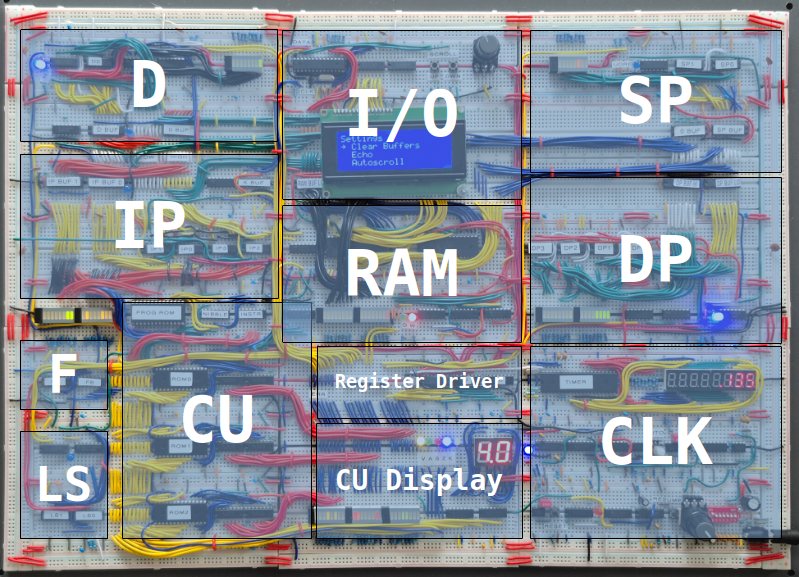
\includegraphics[width=0.8\linewidth]{img/computerparts}
    \caption{Location of the modules on the prototype}
    \label{fig:prototypeb}
  \end{subfigure}
  \caption{}
  \label{fig:prototype}
\end{figure}

%%%%%%% CLOCK

\subsection{Clock} \label{sec:clock}
\begin{figure}[H]
  \centering
  \includegraphics[width=0.6\textwidth]{img/clockmodulecloseup}
  \caption{Close up of the Master Clock and Reset/Resume Modules.}
  \label{fig:masterclockcloseup}
\end{figure}

\subsubsection{Overview}
The clock module is located at the bottom right of the computer and is responsible for providing a heartbeat to (most of) the modules. The core design of the clock, based around a 555 timer in astable mode, is taken directly from Ben Eater's 8-bit computer video's \cite{beneater}. The output frequency can be set using an array of DIP-switches to select the capacitor of an RC-circuit for coarse control and a 10K linear potentiometer for fine control. Two additional 555 timers are used to debounce both the pushbutton for the manual clock and the latching push button which acts as a select between the two modes, as per Ben's design. 

The frequency of the astable 555 is halved by sending it through a JK flip-flop to ensure a perfectly symmetric duty cycle, then fed into a 74LS123 monostable multivibrator to produce two short 200ns pulses: one on the rising and another on the falling edge the output of the flip-flop. This results in two sets of clean signals at constant intervals. On the first pulse (rising edge of the output of the flip-flop), control signals are loaded from the microcode EEPROMs into a set of registers (74LS173) that buffer these control signals for stability; even when the inputs to the EEPROM address-pins change during execution of an opcode, this will not affect the control signals presented at the modules. The second pulse (generated by the falling edge of the flip-flop) is used as a clock to the modules; this is when the modules execute their command, like loading a value into RAM or incrementing the contents of a register. This approach guarantees a clean division between setting the control signals and clocking the modules. Figure \ref{fig:clocktiming} shows the timing diagram for the different signals discussed above.

\begin{figure}[H]
  \centering
  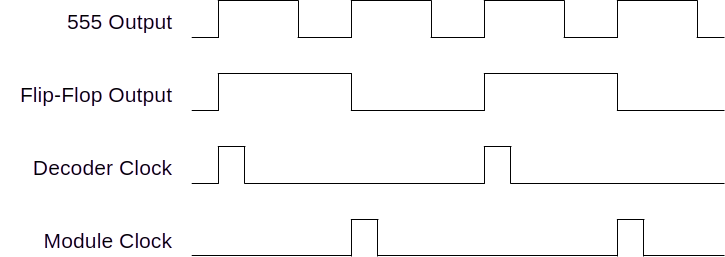
\includegraphics[width=0.6\textwidth]{img/clocktiming}
  \caption{Timing diagram for the clock signals.}
  \label{fig:clocktiming}
\end{figure}

\paragraph{Frequency Control.} The frequency of the master clock can be set using DIP switches to select the capacitor-value and a 10K potentiometer to select the resistance of the RC circuit connected to the 555 timer. The capacitor, in conjunction with a fixed 2K resistor, sets a broad range (lower capacitance corresponding to higher frequencies) while the potentiometer is used fine-grained selection of the frequency within this range. This potentiometer is wired in series with a 1K resistor to ensure stability when the potentiometer resistance drops toward zero. Table \ref{tab:frequencycontrol} shows the frequency-ranges available for each of the currently selected capacitors. These values have been measured \emph{after} the flip-flop (so the actual frequency of the 555 timer is around double the frequencies displayed in table \ref{tab:frequencycontrol}). Having a broad range of frequencies available makes it possible to run at very low speeds for educational purposes, or at very high speeds for complicated, long running algorithms.

\begin{table}
  \centering
  \begin{tabular}{c|r|r}
    Capacitance (F) & $f_{min}$ (Hz) & $f_{max}$ (Hz) \\ \hline
    $10^{-5}$  & 5 & 15 \\
    $10^{-6}$  & 40 & 140 \\
    $10^{-7}$  & 500 & 1,500 \\
    $10^{-8}$  & 5,000 & 14,000 \\
    $10^{-9}$  & 19,000 & 55,000 \\
    $10^{-10}$ & 38,000 & 108,000 \\
    $10^{-11}$ & 90,000 & 270,000 \\
  \end{tabular}
  \caption{Frequency ranges for each of the capacitors (approximate).}
  \label{tab:frequencycontrol}
\end{table}

\paragraph{Frequency Display:} To be able to see the clockfrequency as well as the instruction-frequency (number of BF instructions executed per second), the module clock (M\_CLK) and INC(IP) signals are connected through a switch to the input of an ICM7226B timer chip \cite{7226B}, which is configured as an 8-digit frequency timer. It drives two 4-digit 7-segment displays at a 1 second interval (the frequency is measured and updated every second). 

\subsection{Reset/Resume} \label{sec:resetresume}
\paragraph{Reset.} The Reset/Resume module is located directly underneath the clock and contains logic necessary to reset the computer (necessary after applying power) or resume the clock after it has been halted. The HLT signal coming from the decoder is latched into a register (74LS173) from which the corresponding output bit is connected to the HLT input of the clock module. When the system is reset (using the reset button) or when the resume button is pressed, the HLT bit is cleared and the clock output is enabled again. This allows for pausing and resuming the computer, effectively adding breakpoints to the code. The reset button itself is debounced in the same way as the manual clock button to ensure a stable transition with a debounce time of around 300ms.

\paragraph{Resume.} The Resume button needs more sophisticated debounce circuitry due to the following scenario: when multiple HLT instructions are seperated by a relatively small amount of other instructions, a pulse in the order of milliseconds (like the reset and pulse debouncers) will be far too long at high clock frequencies. The resume-signal will still be high when a second (or third, fourth, ...) HLT instruction is encountered, causing control flow to simply skip over these instructions. To remedy this situation, a debouncing circuit is required that first produces a pulse of equal width of the clock pulses (Figure \ref{fig:clocktiming}), followed by a guaranteed period where the signal is low, even when the button bounces after the pulse. This is achieved by creating a feedback loop between the two monostable vibrators present on the 74LS123. The first one will produce a 200ns pulse on the rising edge of the button. This pulse is sent to the reset of the register that holds the HLT signal in order to clear it, but is also connected to the second monostable vibrator. When the initial (short) pulse goes low, the second vibrator generates a much longer pulse that is connected to the reset-input of the first one, making sure it cannot be re-activated for some time. By selecting a 680K resistor and a 4.7$\mu F$ capacitor, a cooldown period of around 1 second is achieved. Figure \ref{fig:resumedebounce} shows a timing diagram to illustrate this process in more detail. 

\begin{figure}[H]
  \centering
  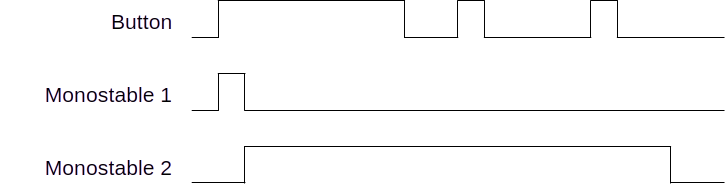
\includegraphics[width=0.6\textwidth]{img/resumedebounce}
  \caption{Timing diagram for the resume debouncer. The output of Monostable 1 is connected to the reset of the register that stores the HLT signal.}
  \label{fig:resumedebounce}
\end{figure}


\subsubsection{Schematic}
Full schematics for the clock module, reset/resume circuitry and the frequency display section are provided on the next pages.
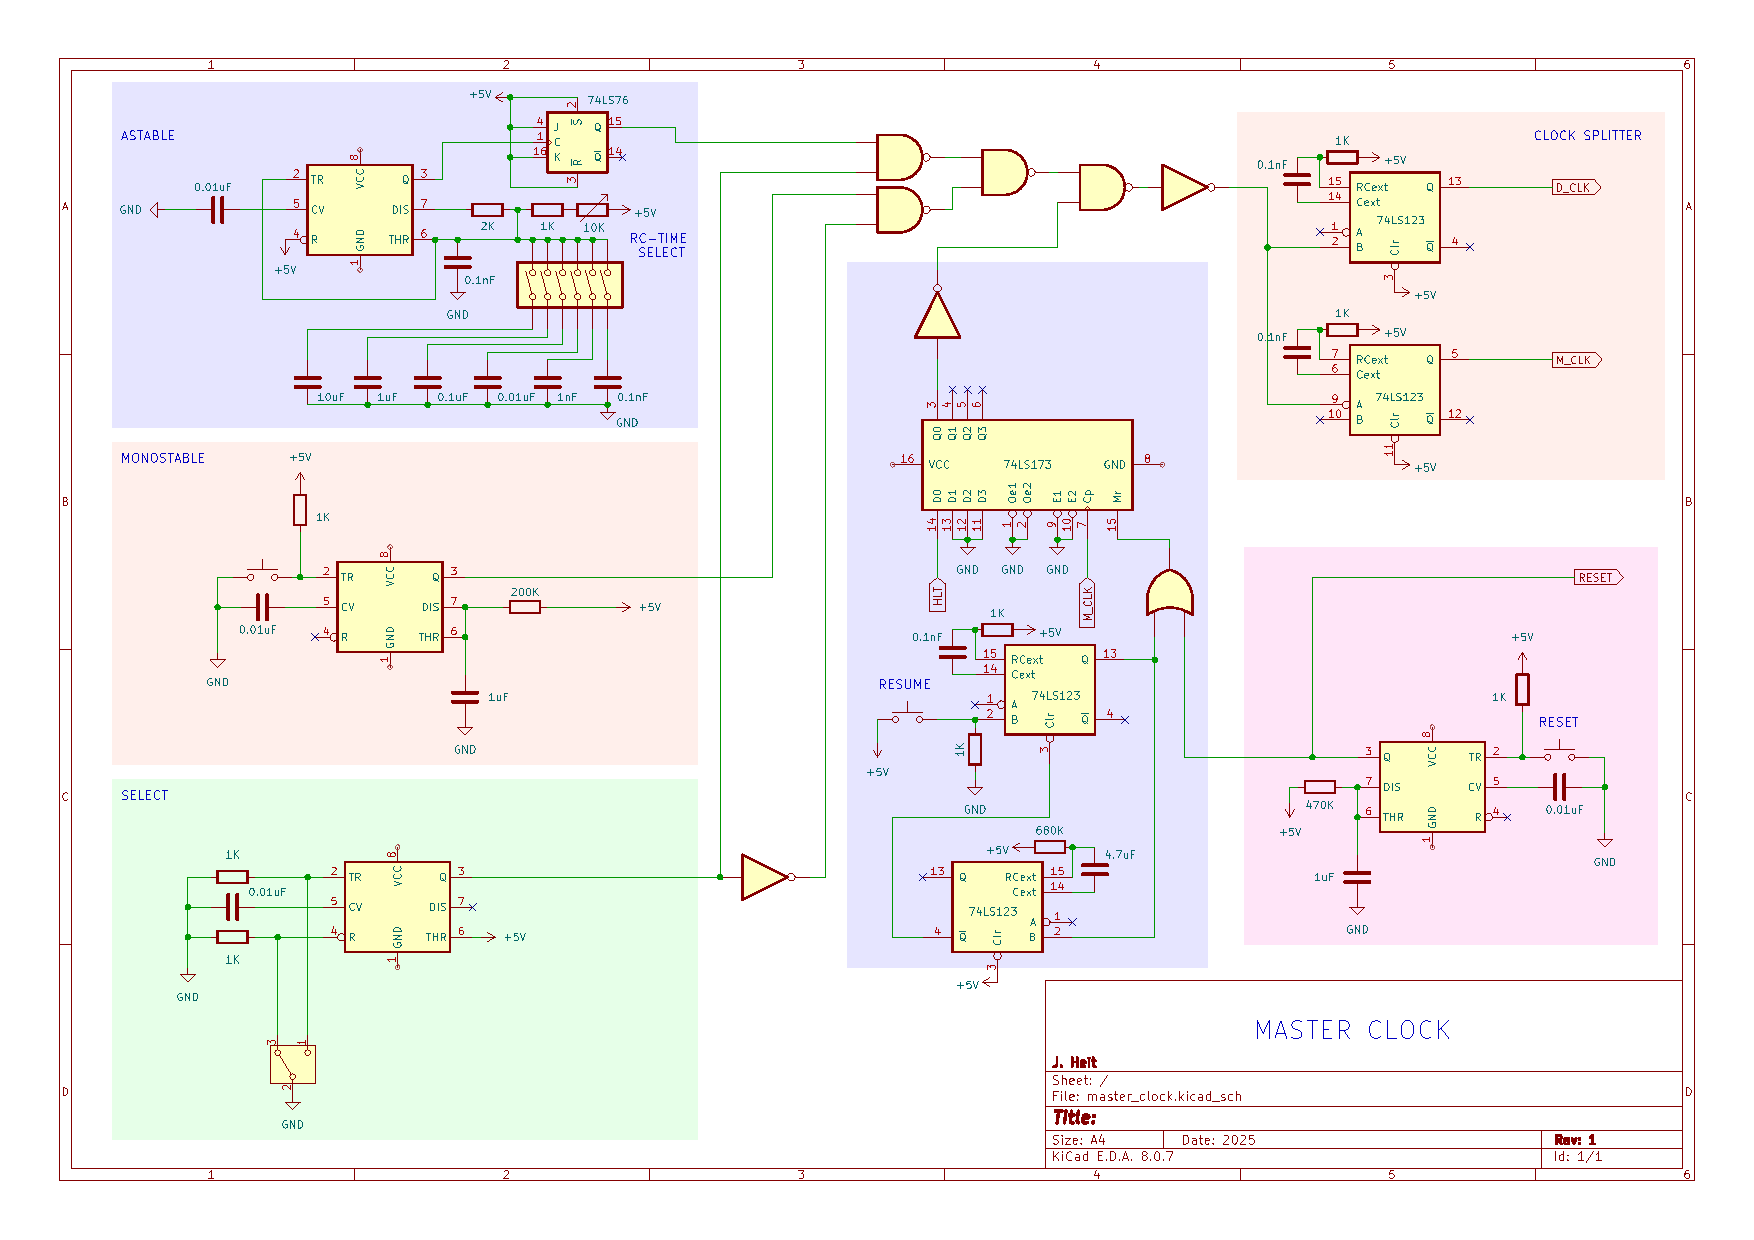
\includepdf[landscape=true]{schematics/masterclock.pdf}
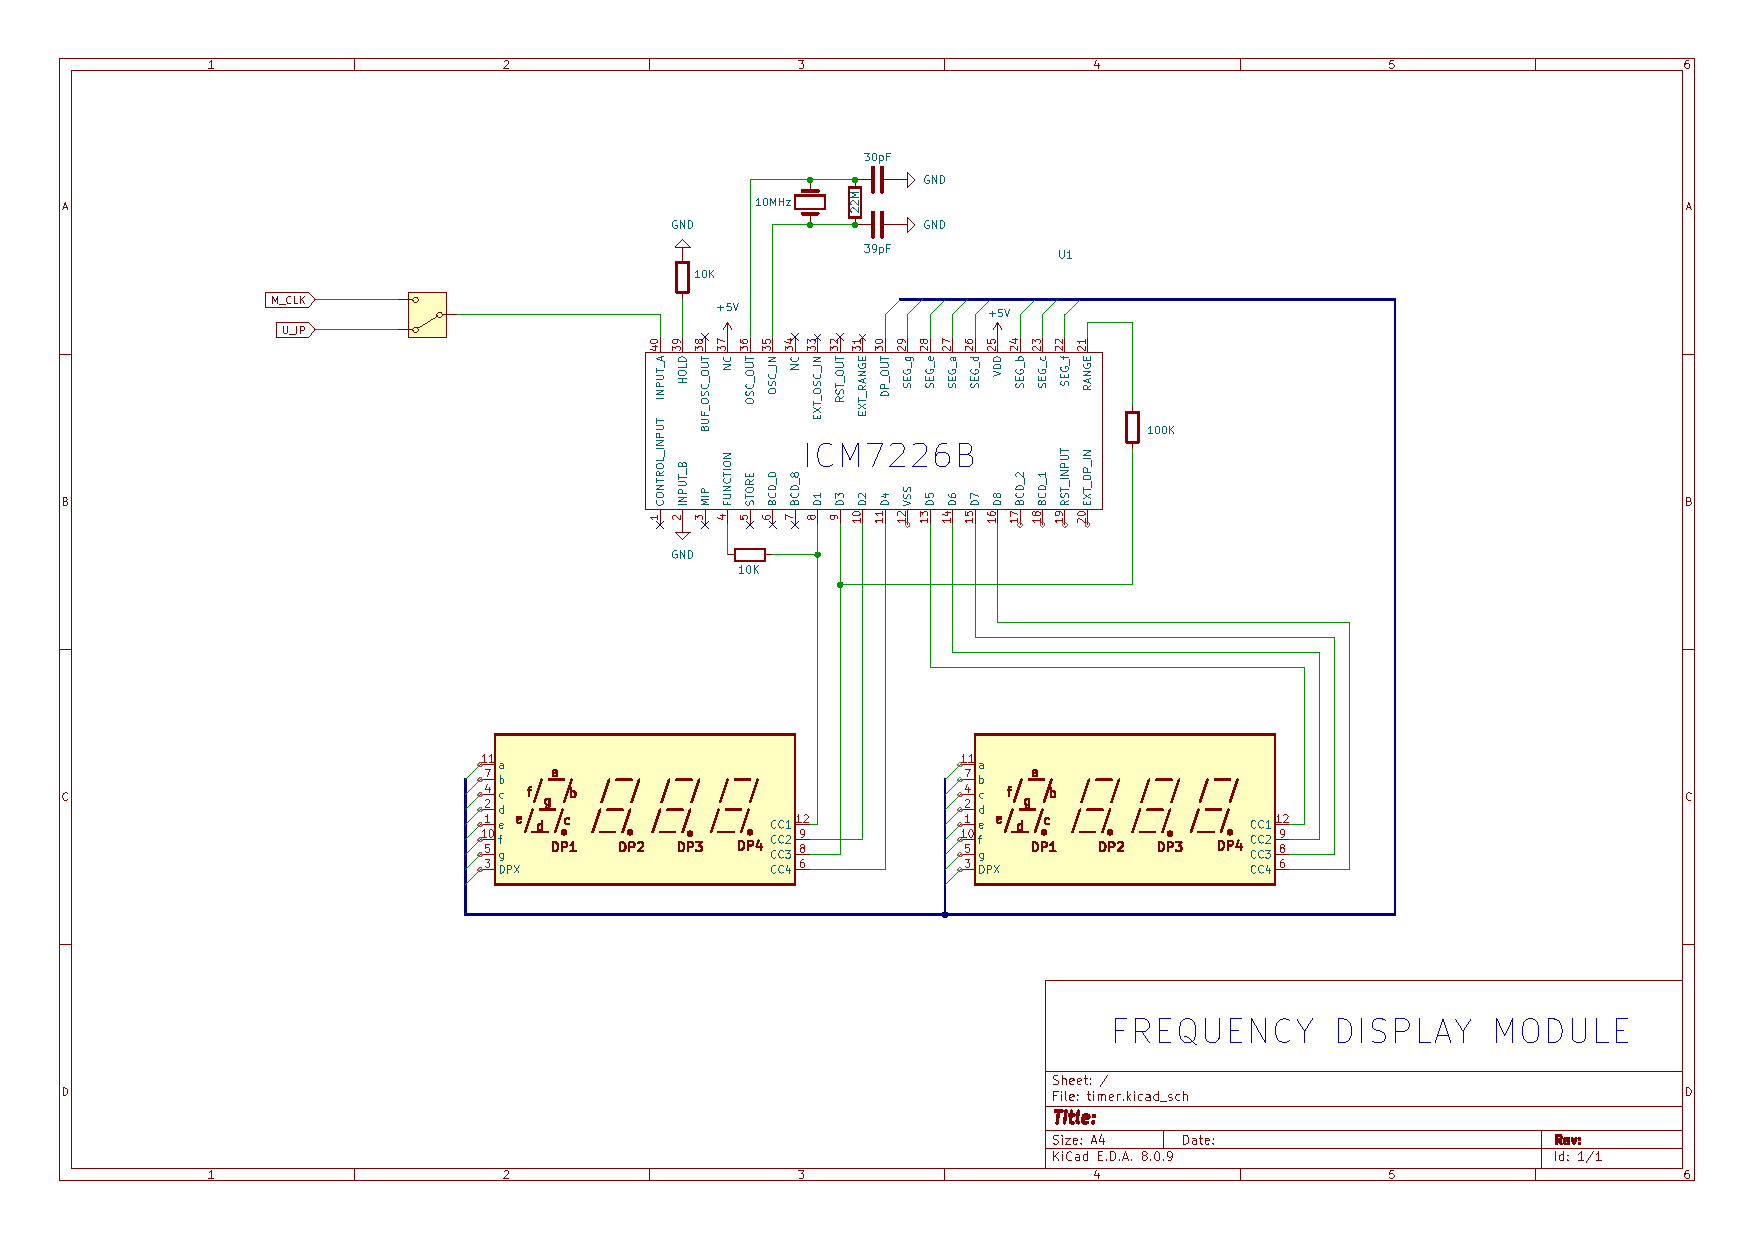
\includepdf[landscape=true]{schematics/frequencydisplay.pdf}

%%%%%%% REGISTER DRIVER

\subsection{Register Driver} \label{sec:implementation:registerdriver}
\begin{figure}[H]
  \centering
  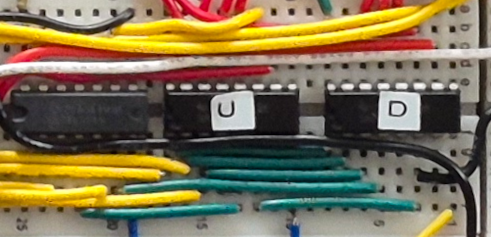
\includegraphics[width=0.6\textwidth]{img/registerdrivercloseup}
  \caption{Close up of the Register Driver Module.}
  \label{fig:registerdrivercloseup}
\end{figure}

\subsubsection{Overview}
The register driver is responsible for driving the U- and D-inputs of the 74LS193 counting registers that are used to implement the D, DP, SP, IP and LS register modules. To increment the '193, its D-input needs to be held high while providing a low pulse to the U-input. As explained in section \ref{sec:architecture:cu}, a centralized driver was used to limit the number of logic IC's necessary to drive the registers and the total number of control signals necessary.

The driver module uses a pair of 74LS138 decoders: one to drive the U-inputs and the other to drive the D-inputs of the '193. The '138 takes 3 address bits (A, B, and C) to select one of 8 outputs (Y0-Y7), which will be pulled low when selected (all other outputs remain high). Two gate-inputs G1 (active high) G2 (active low) are used to enable the outputs of the chip; the selected output is activated (pulled low) only when both gates are active. This is very convenient given the fact that the 74LS193 needs a low pulse to increment or decrement its value:
\begin{itemize}
\item The register-selects signals RS0, RS1 and RS2 are connected to A, B, and C to select the required output.
\item The INC and DEC signals are connected through inverters to the G2 gate.
\item The module-clock signal is connected to G1: when pulsed, the selected output will produce a pulse that is effectively an inverted clock pulse (high-low-high) which is exactly what the '193 expects. 
\end{itemize}

\subsubsection{Schematic}
A full schematic is provided on the next page.
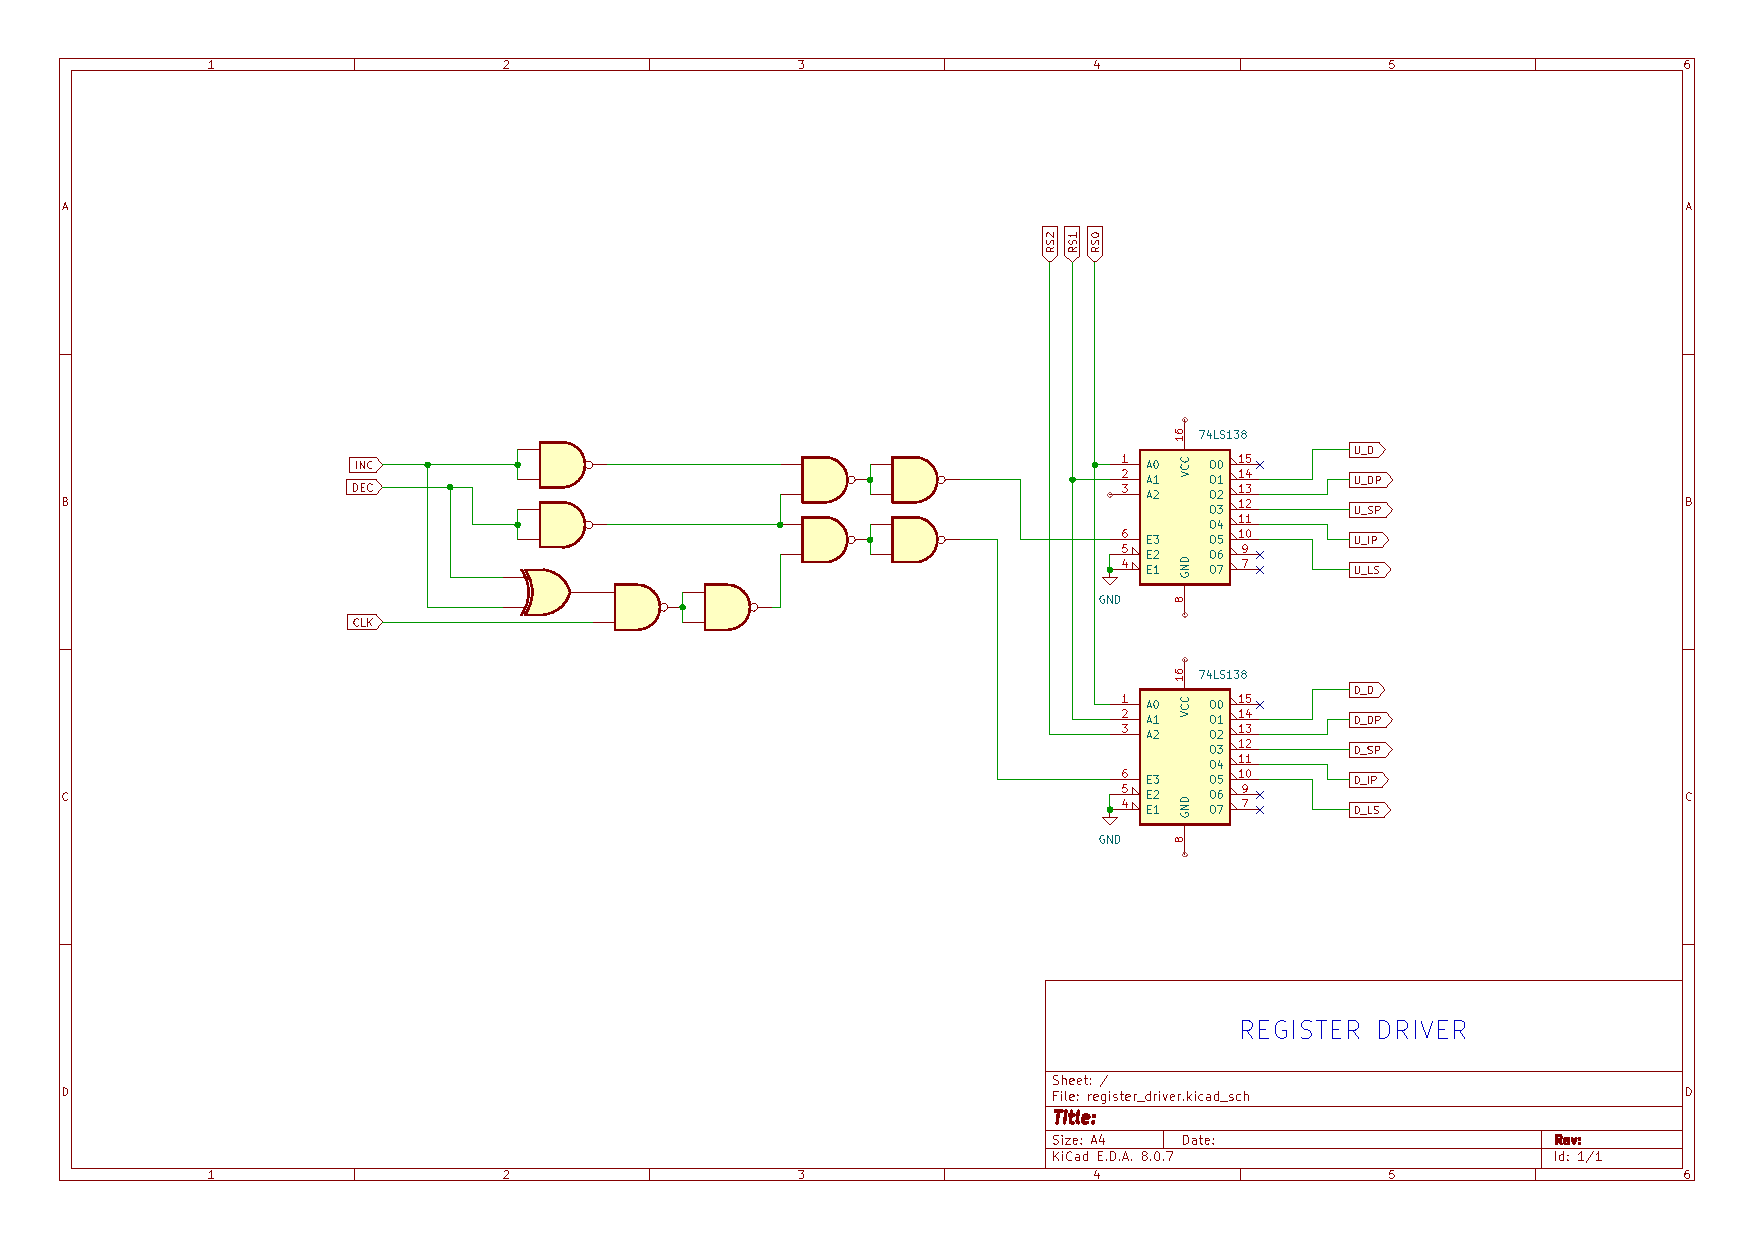
\includepdf[landscape=true]{schematics/registerdriver.pdf}

%%%%%%% DATA POINTER REGISTER

\subsection{DP Register} \label{sec:implementation:dp}
\begin{figure}[H]
  \centering
  \includegraphics[width=0.6\textwidth]{img/dpregistercloseup}
  \caption{Close up of the Data Pointer Register Module.}
  \label{fig:dpregcloseup}
\end{figure}

\subsubsection{Overview}
The DP Register Module is the module that is responsible for managing the data-pointer; it contains a 16-bit value that is connected to the address bus of the RAM and points to the memorycell currently pointed to by the BF-pointer. The value is stored across four 74LS193 binary counters that are chained together (each holding 4 bits), making it possible to address a total of $2^{16}=65,536$ different memory cells. The DP is connected to the register driver at address 2 (0b010, see Table \ref{tab:registers}) and as such can be incremented or decremented when the program hits a \texttt{>} or \texttt{<} respectively. The outputs of each '193 are connected to the address bus through a pair of tristate buffers (74LS245) to prevent bus contention with the stack pointer; see below (Enabling Ouput) for more information on the enable-signal.

\paragraph{Reset Vector.} Since the data section in RAM starts at 0x0100 (0x0000 through 0x00ff are reserved for the stack), this is the value that the register should start at right after booting up the system (all other registers start out with an initial value of zero). To achieve this, the global reset line of the system is connected to the reset pin of the 193's corresponding to nibbles 0, 1 and 3, but to the load-pin of nibble 2, who's inputs have been hardcoded to 0b0001 (0x1). This register is also special in the sense that it is the only register that needs to reset at runtime (through the CLR\_DP signal), without resetting any of the other modules. After all, after initializing its memory to 0 by looping through (part of) its addressable space, the DP needs to be brought home to the start of the datasection before the main program starts (see also Sections \ref{sec:sequences:init} and \ref{sec:sequences:home}). The global RESET signal is therefor OR'd with the CLR\_DP signal before going to the reset (and load) pins of the IC's.

\paragraph{Enabling Output.} Perhaps somewhat confusingly, the schematic (see below) shows that the SP\_EN signal is used to enable the buffers. Because the DP shares the address-bus with only the stack pointer (SP) -and their outputs should be mututally exclusive- the same signal can be used to enable and disable their respective buffers: when the stack pointer is enabled, the data pointer should be disabled and vice versa. Given that the output-enable-pin of the 74LS245 is active low, the SP\_EN signal can be fed directly into the enable-pin of the DP buffers. On the side of the SP, the same signal goes through an inverter before going into the enable-pin of its respective buffer. By default, when the SP is not enabled, the DP will provide its address to RAM. The address-bus will therefore never be left floating, which has the nice side-effect of always being able to visually see the current value in RAM by the LED's connected to its outputs. 

\subsubsection{Schematic}
A full schematic is provided on the next page.
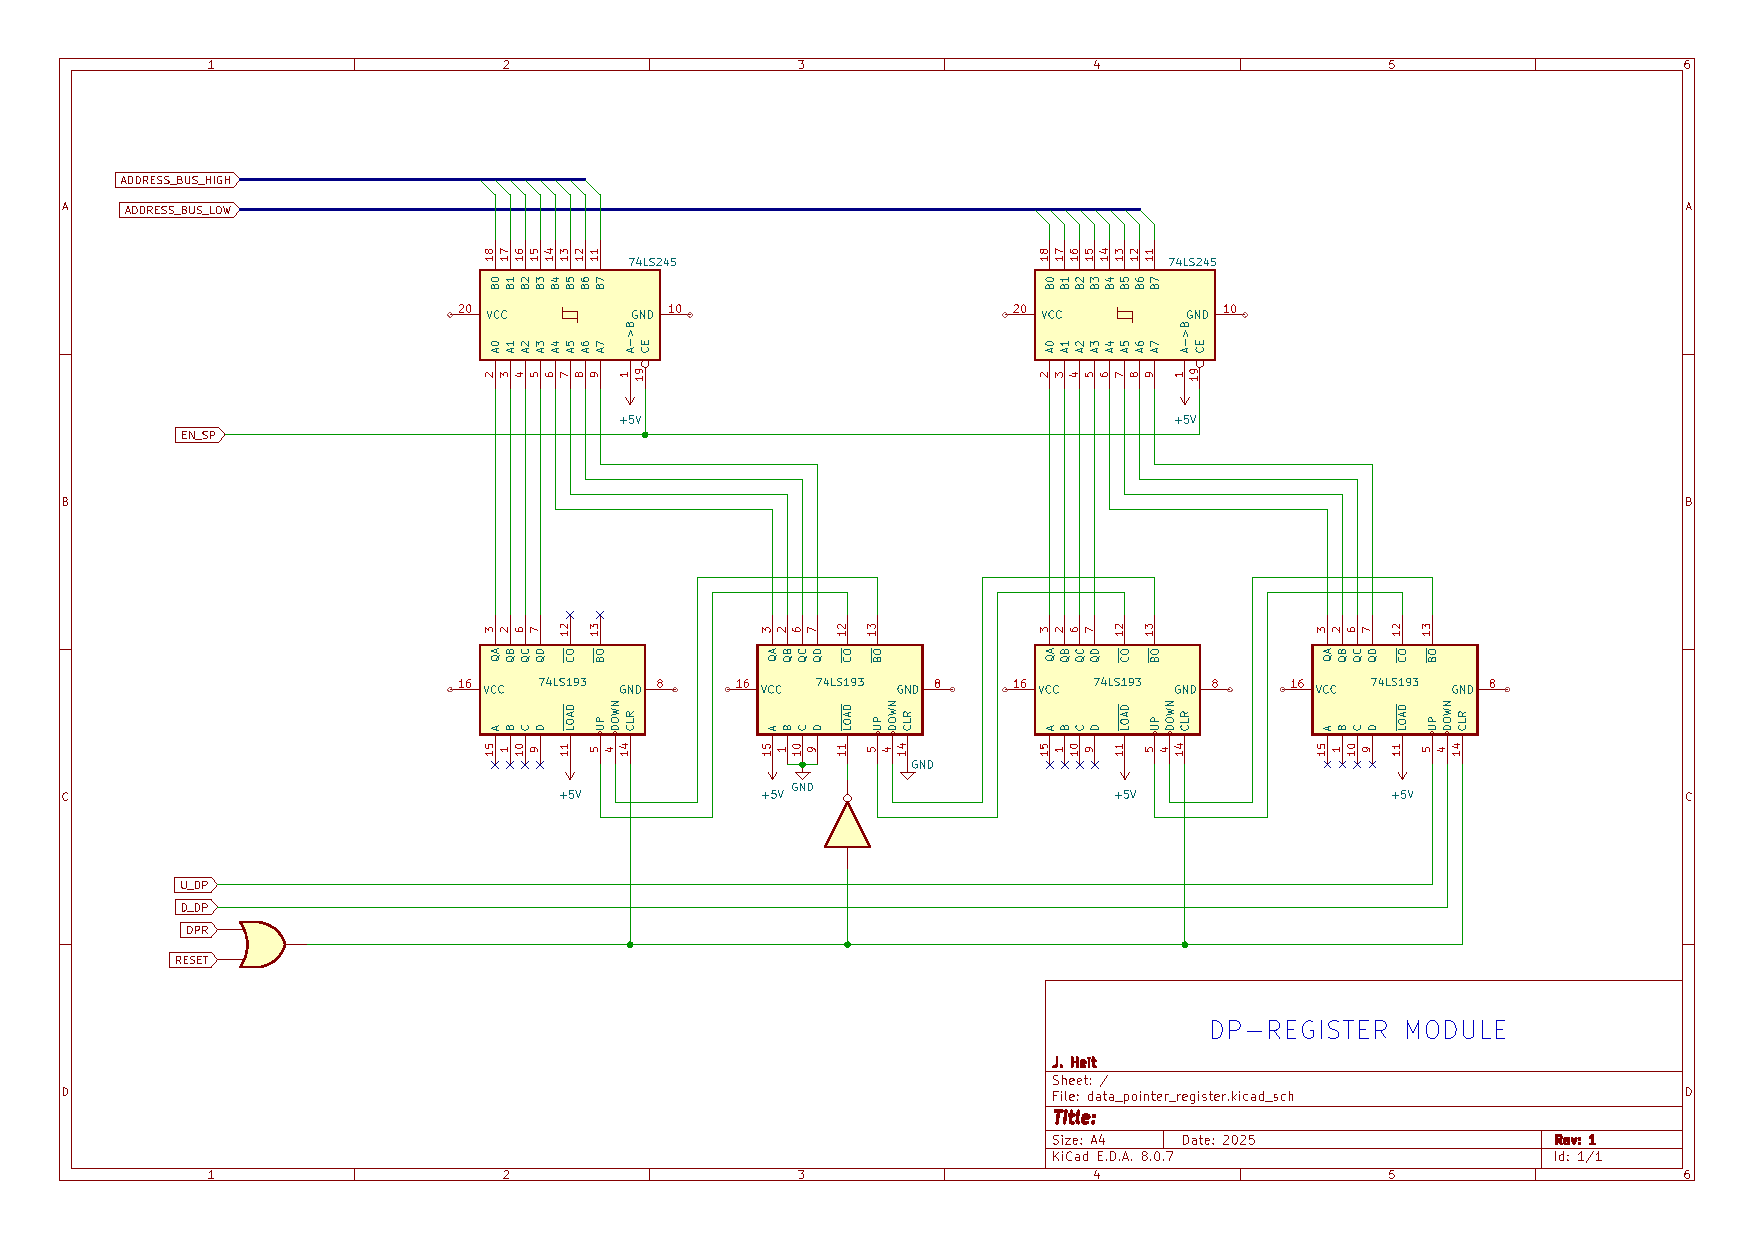
\includepdf[landscape=true]{schematics/datapointerregister.pdf}

%%%%%%% DATA REGISTER

\subsection{D Register}
\begin{figure}[H]
  % TODO: add annotations to the image
  \centering
  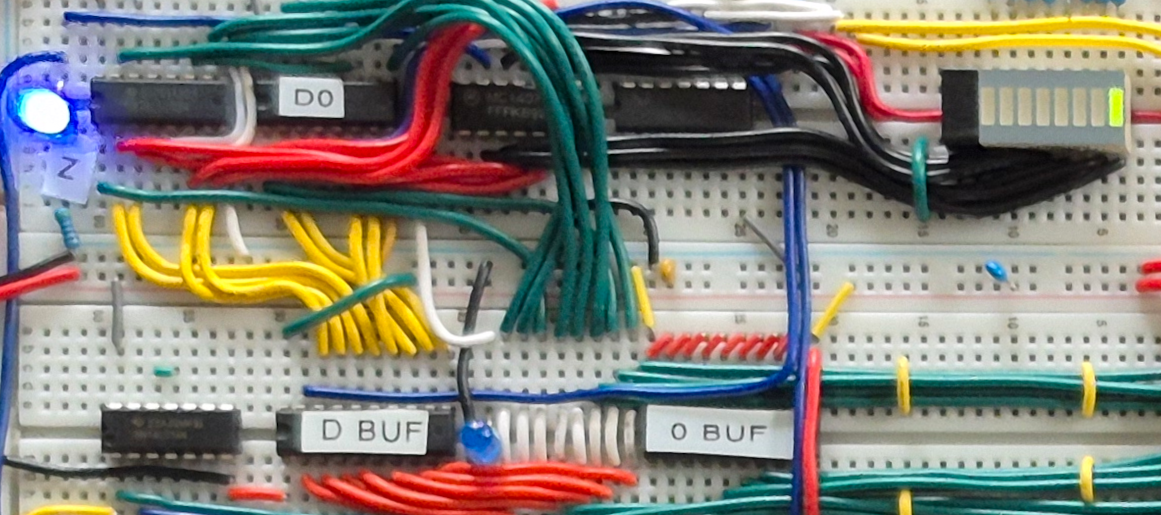
\includegraphics[width=0.45\textwidth]{img/dregistercloseup}
  \caption{Close up of the Data Register Module.}
  \label{fig:dregcloseup}
\end{figure}

\subsubsection{Overview}
The data register (D) holds (a copy of) the value in memory currently pointed to by the datapointer (DP). In the computer, it is located in the top left corner. Like the DP, it is implemented using 74LS193 counting registers and driven by the register driver described in Section \ref{sec:implementation:registerdriver} at address 1 (0b001, see Table \ref{tab:registers}). Since the data is only 8-bits in size, no more than two '193 chips have to be chained together to create the 8-bit register. 

\paragraph{Enabling Output. } The outputs of the '193s are buffered by a single 8-bit tristate buffer (74LS245) before being connected to the databus. Because the databus is 16-bit wide (necessary to store IP-values on the stack), the high-byte is set explicitly to 0 when D is enabled by a second buffer that always outputs zero's. Storing nonzero values in the high-byte of the datasection would not have any consequences for the computation, but would be visually confusing. The buffers are set to output-mode only (even though the register is able to read from the bus as well) because the 193 chips have seperate pins for incoming and outgoing data. The incoming data is read from the bus directly without needing to go through a buffer.

\paragraph{Z-Flag.} This module also produces the Z flag, indicating that it is currently containing the value 0. This is achieved by connecting its outputs through an 8-input NOR gate (MC14078B). The output of this gate is then connected to the FB flag register where it can be latched in by the CU in order to determine the next course of action.

\paragraph{Loading Data.} Because the '193 loads asynchronously, the clock has to be gated with the LD\_D signal through a NAND gate in order to load synchronously with the clock when the LD\_D signal is high (the load-pin on the '193 is active low). The necessity of a NAND gate meant it was easier to also implement any inverters needed in the circuit in terms of NAND gates.


\subsubsection{Schematic}
A full schematic is provided on the next page.
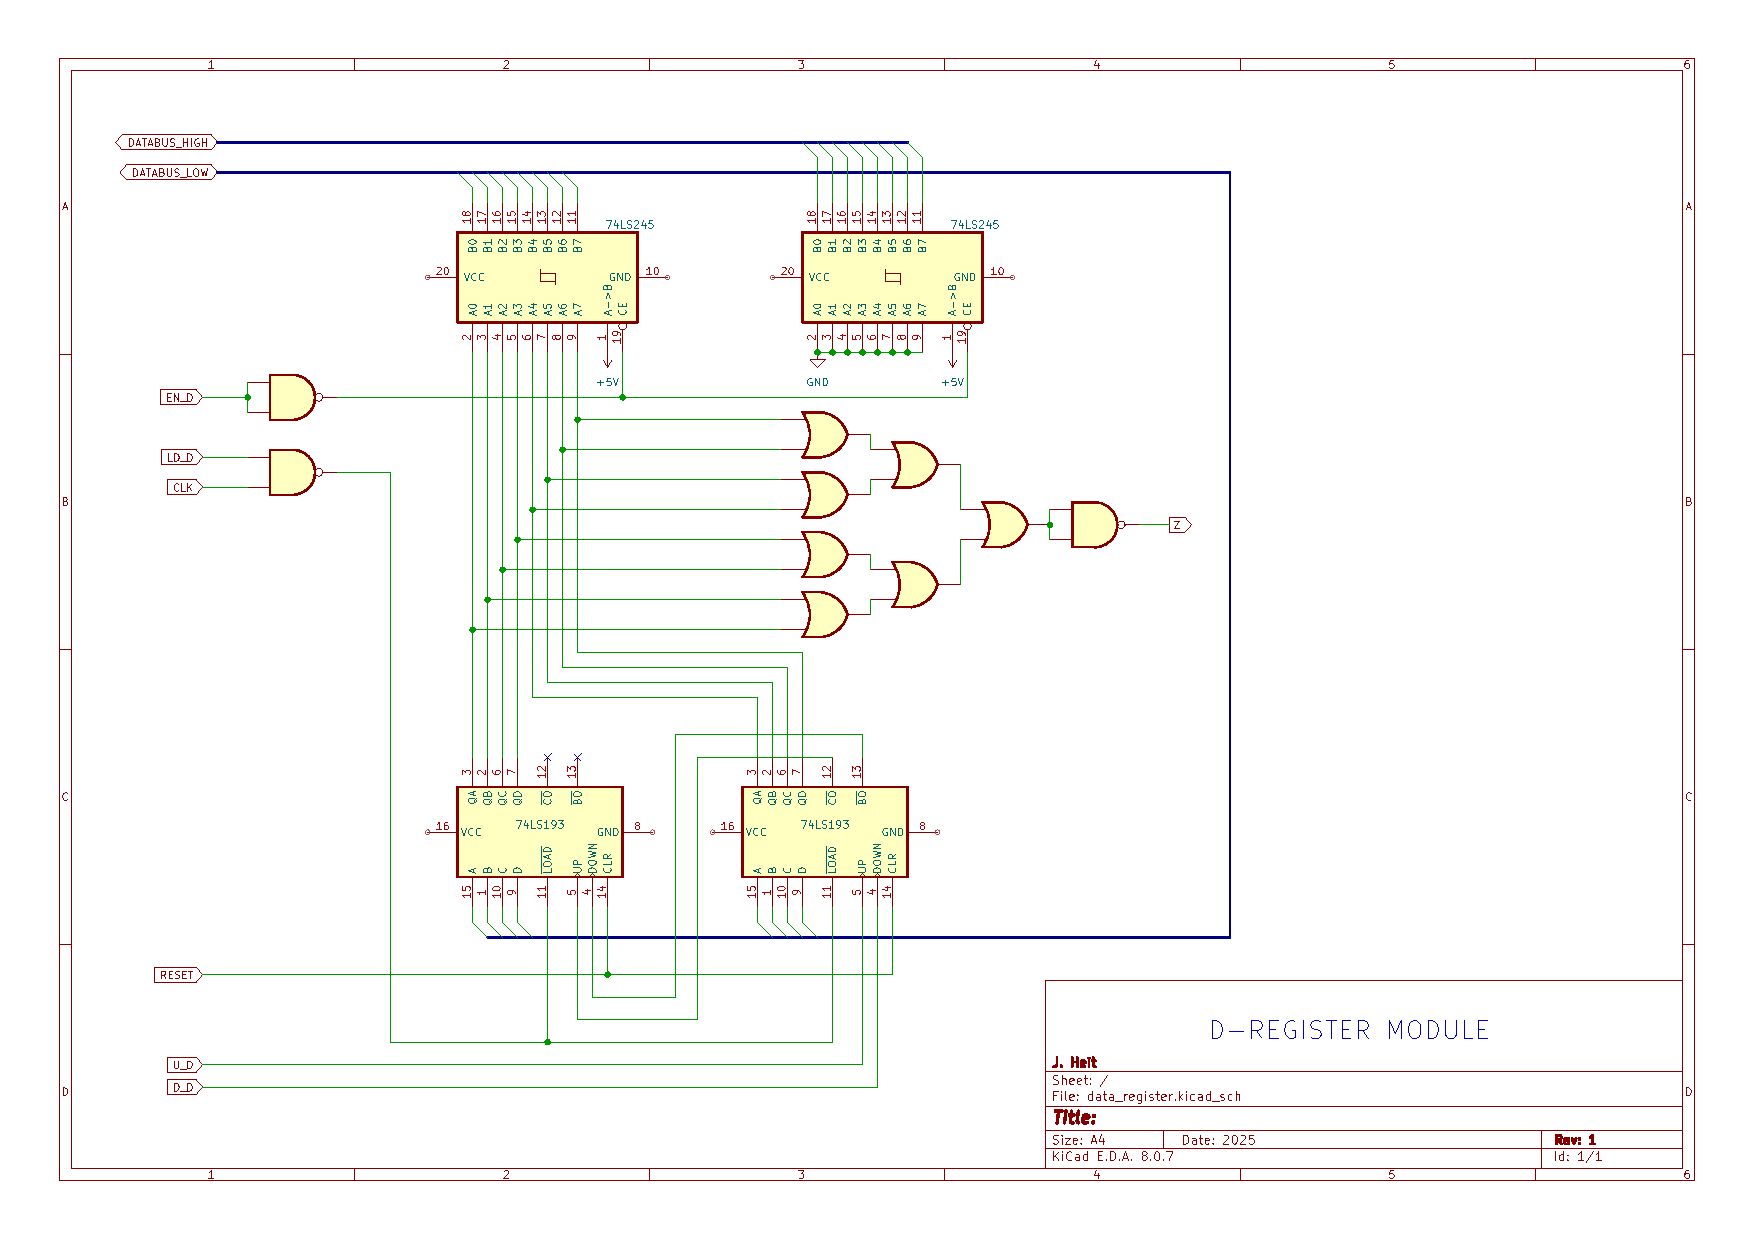
\includepdf[landscape=true]{schematics/dataregister.pdf}

%%%%%%% INSTRUCTION POINTER REGISTER

\subsection{IP Register}
\begin{figure}[H]
  \centering
  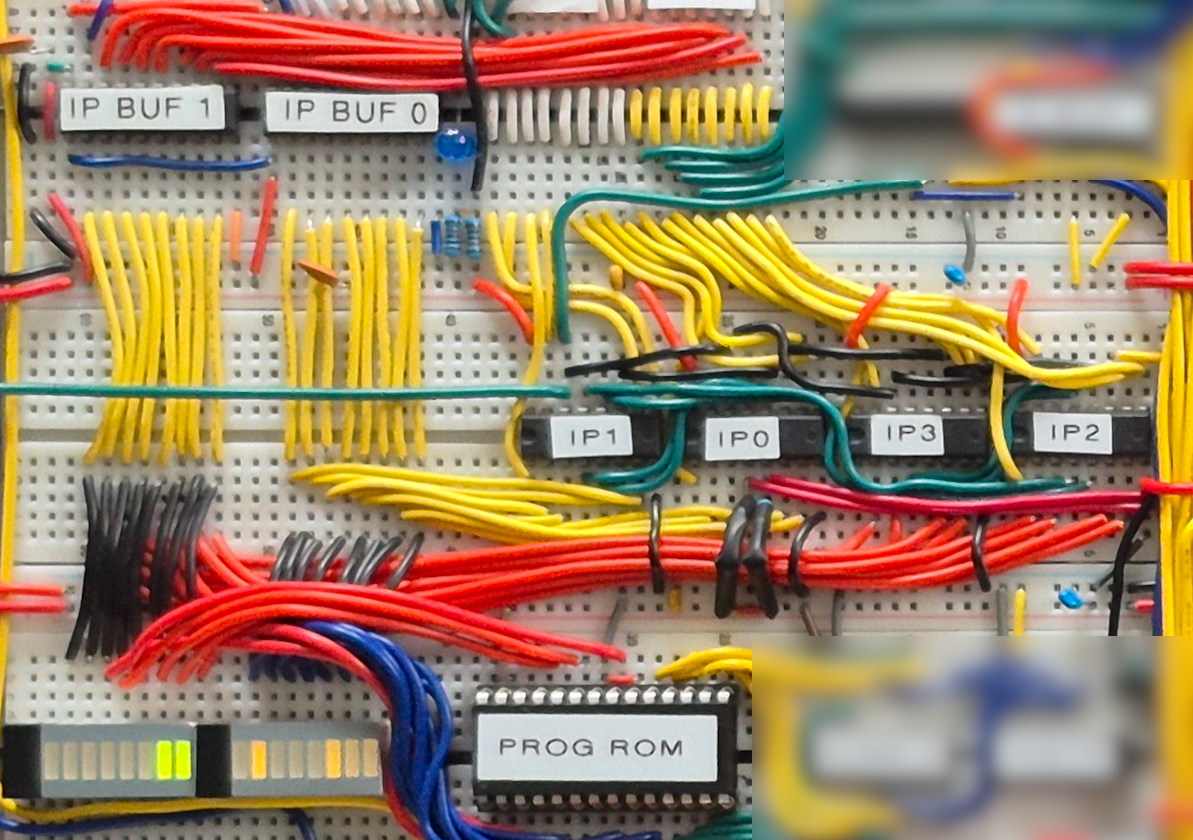
\includegraphics[width=0.6\textwidth]{img/ipregistercloseup}
  \caption{Close up of the Instruction Register Module.}
  \label{fig:iregcloseup}
\end{figure}

\subsubsection{Overview}
The instruction pointer register holds a 16-bit value representing the address of an instruction in the program-ROM (implemented using an EEPROM chip (AT28C64B)). The size of the available address space in program-memory is $2^{14}$ instructions, so the two uppermost bits (bits 14 and 15) of the IP are left unused.

\paragraph{Forbidden Decrement.} The IP, like the D and DP registers, is driven by the Register Driver at address 4 (0b100), but should in principle never be decremented; it either moves to the right (next instruction) or jumps back by loading a value from the databus. Its inability to move left (decremented) is not enforced by the hardware itself, but should be taken care of by the microcode implementation.

\paragraph{Reading and Writing Data.} The IP is connected to the databus through two tristate buffers (74LS245) to avoid bus contention with the DP and IO-module. It is connected to this bus in order to write its value to the stack when a loop is entered. When exiting from a loop, a value is read back into the register through a direct connection to this bus (without going through a buffer). Because loading is done asynchronously on the '193, the load signal is NAND'ed with the clock to make loading synchronous again.

\subsubsection{Schematic}
A full schematic is provided on the next page.
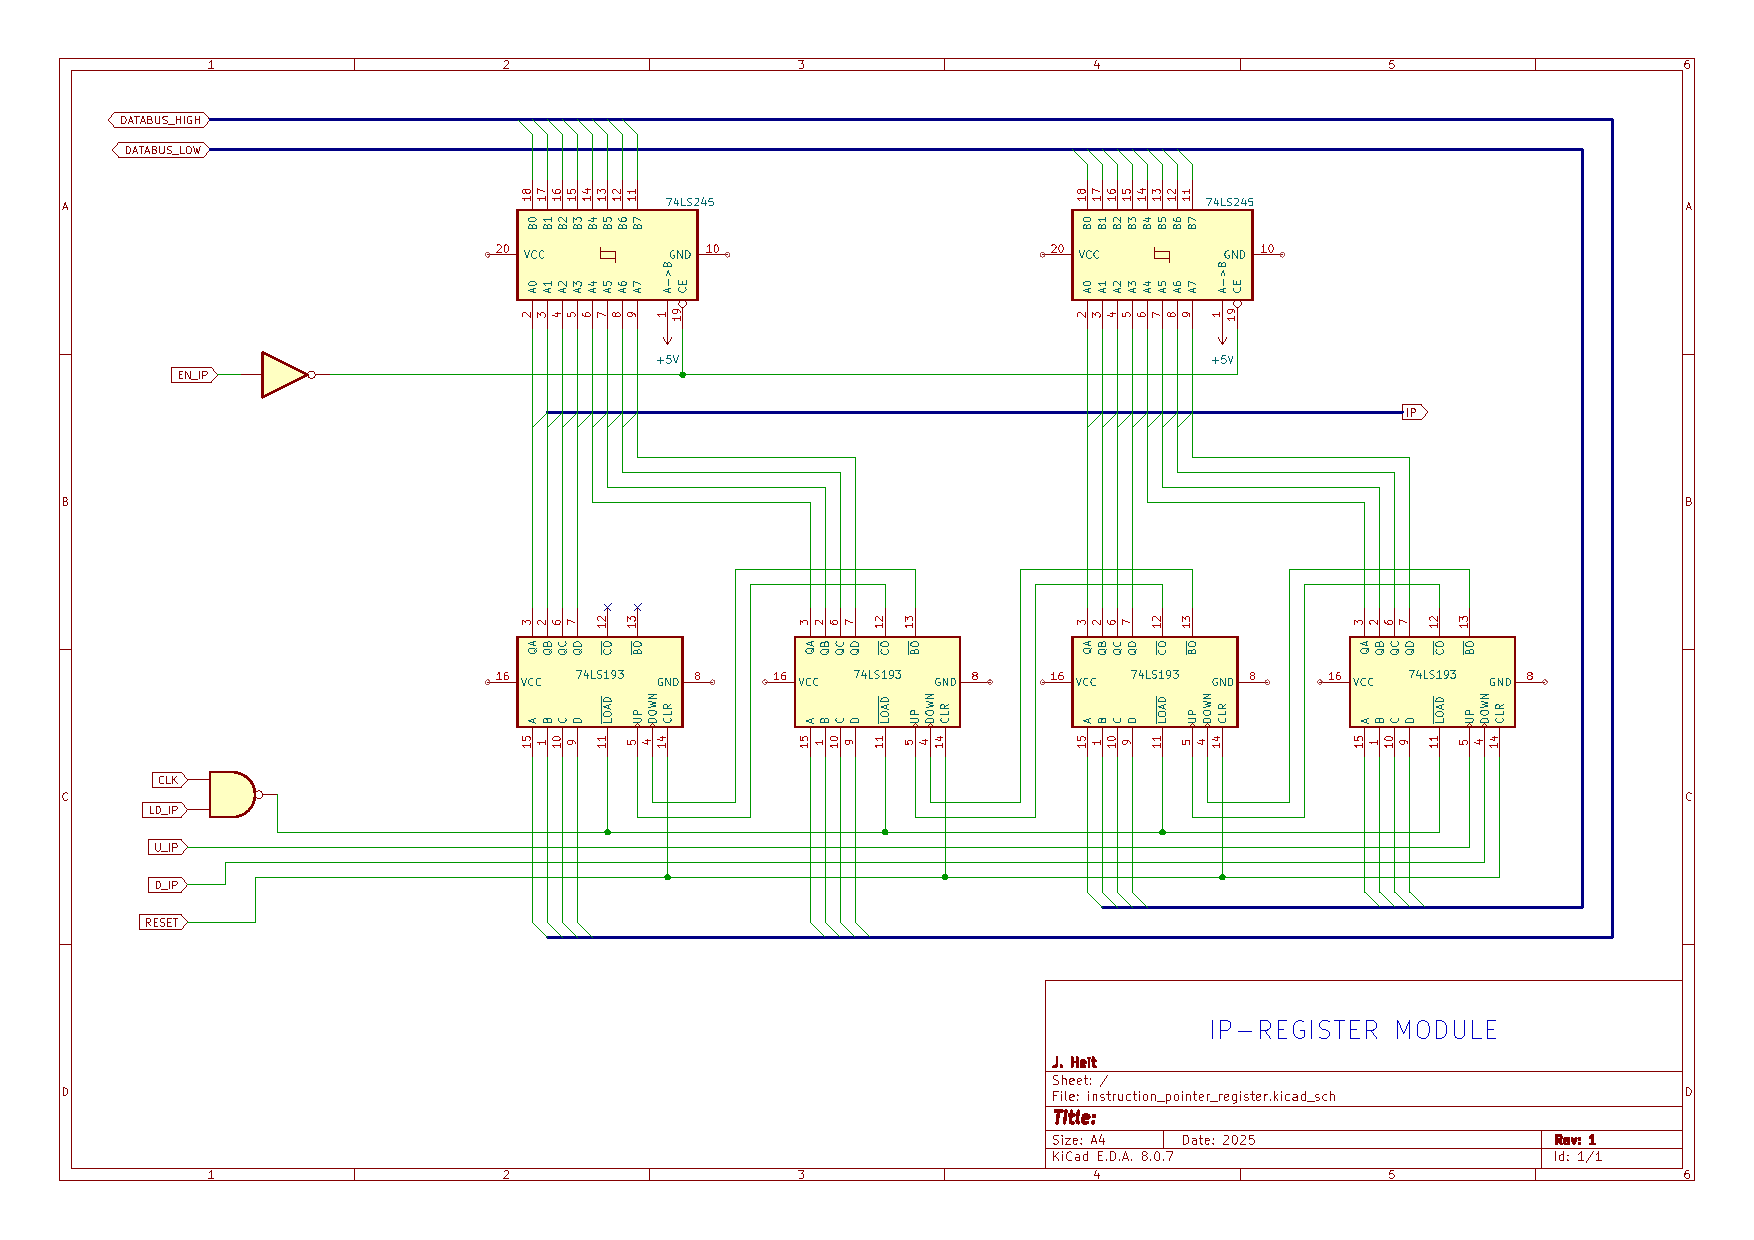
\includepdf[landscape=true]{schematics/instructionpointerregister.pdf}

%%%%%%% STACK POINTER REGISTER

\subsection{SP Register}
\begin{figure}[H]
  \centering
  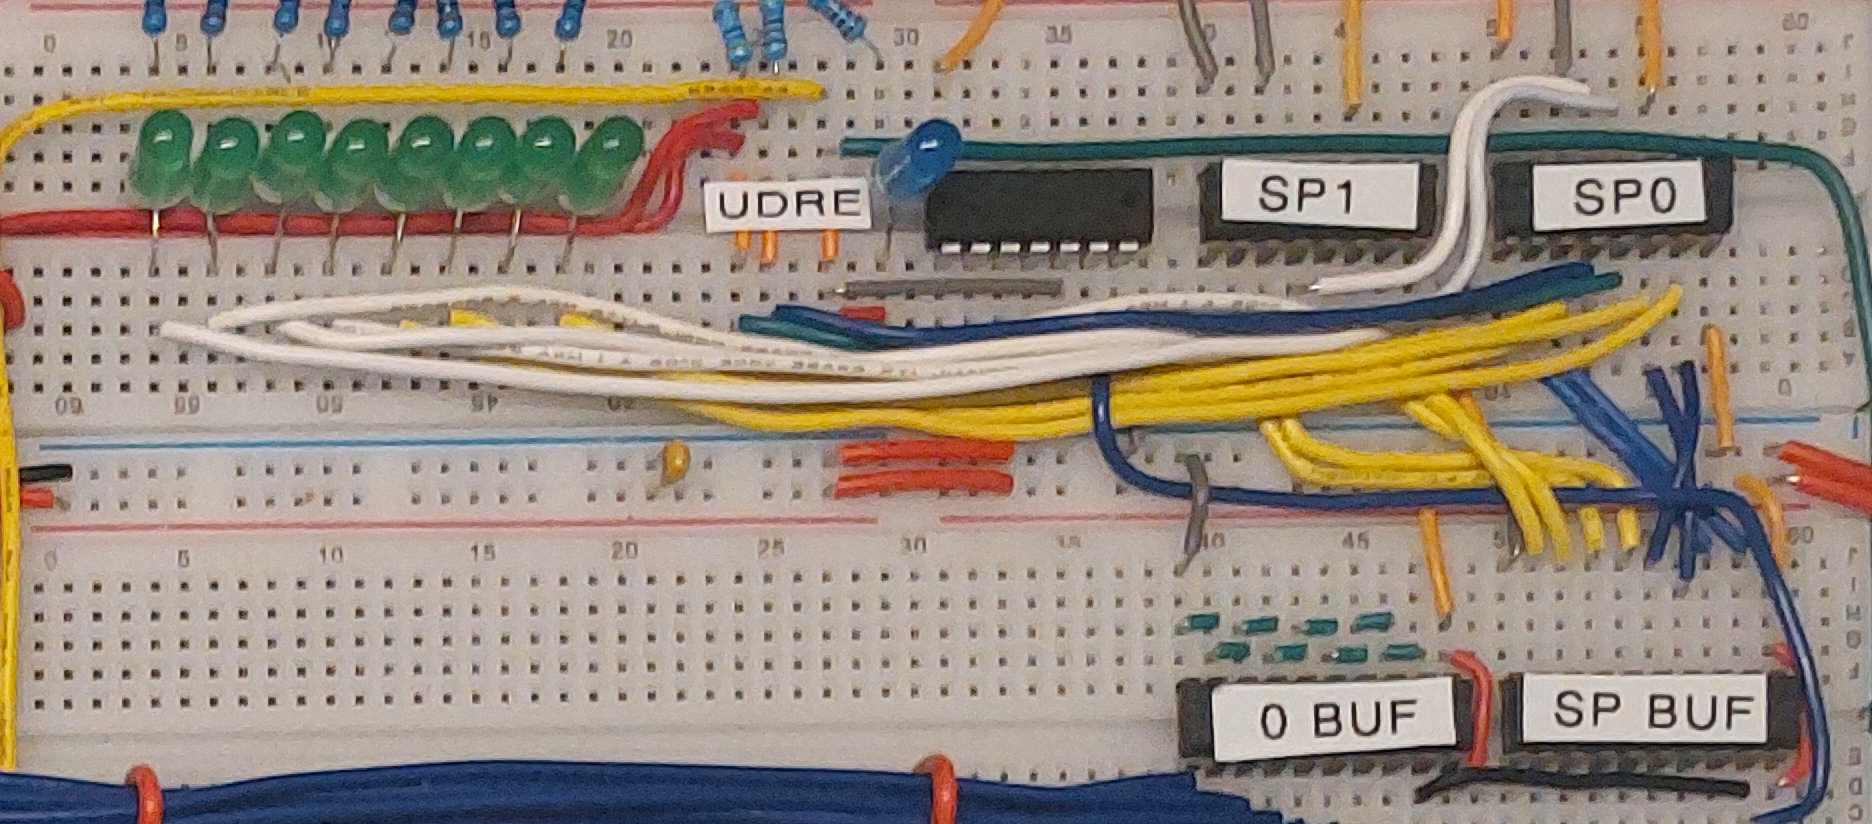
\includegraphics[width=0.6\textwidth]{img/spregistercloseup}
  \caption{Close up of the Stack Pointer Register Module.}
  \label{fig:spregcloseup}
\end{figure}

\subsubsection{Overview}
The stack pointer (SP) holds an 8-bit value in the range 0x00 - 0xff, which corresponds to addresses within the stack-space of RAM, where IP values can be stored and loaded from when the system sees the \texttt{[} and \texttt{]} loop-instructions. When a loop is entered, the IP register stores its value on the stack at the address pointed to by the SP. The SP then increments its value, ready for the next value to be stored on the stack when a nested loop is encountered. It is therefore implemented using the 74LS193 binary counter and connected to the register driver at address 3 (0b011). The SP module is connected to the same RAM address bus as the DP, which means it should go through a tristate buffer to avoid bus contention. As mentioned before (\ref{sec:implementation:dp}), the SP buffer shares its enable-line (though inverted) with the DP. A second buffer that, when enabled, only outputs zero's on the address-bus is used to make sure that only the stack is addressed by the SP and no accidental reads or write happen in the datasection. 


\subsubsection{Schematic}
A full schematic is provided on the next page.
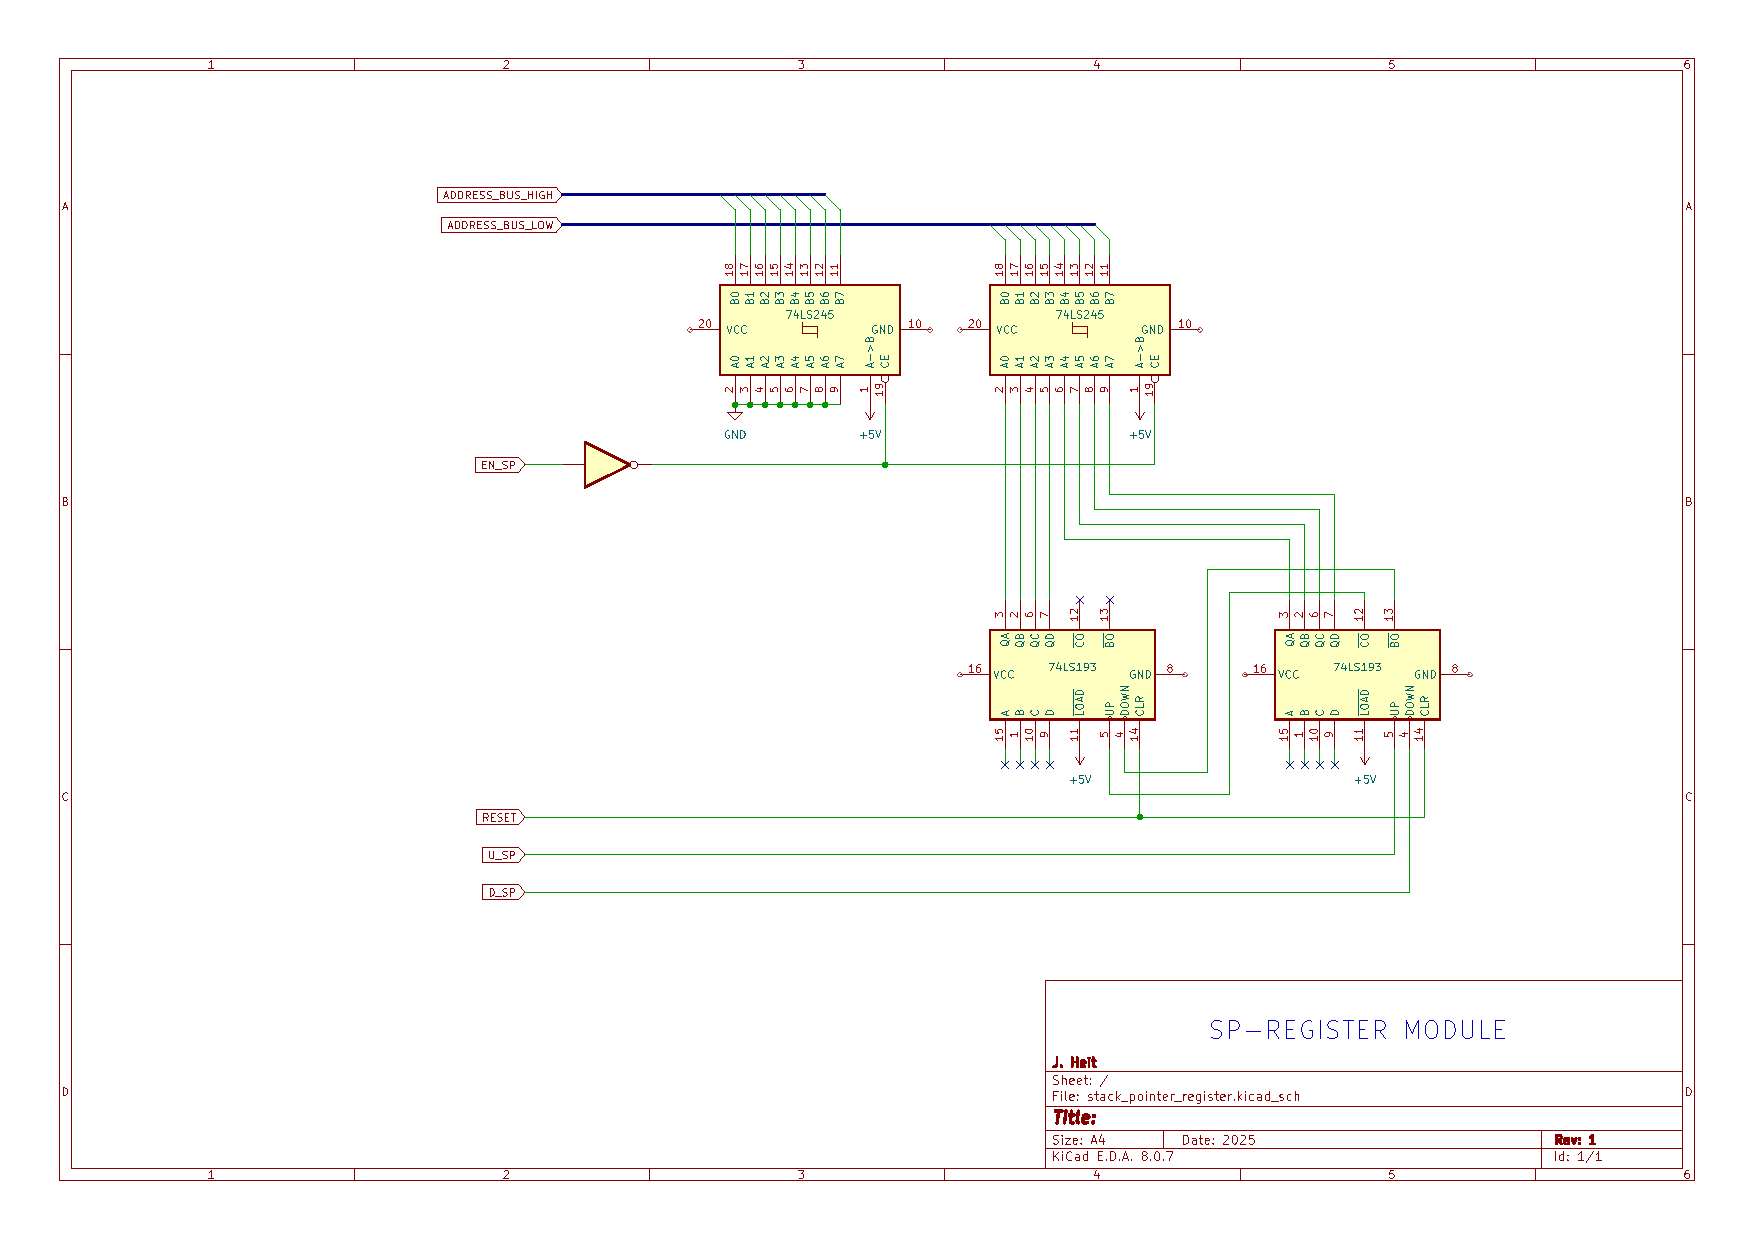
\includepdf[landscape=true]{schematics/stackpointerregister.pdf}


%%%%%%% LS Register

\subsection{LS Register}
\begin{figure}[H]
  \centering
  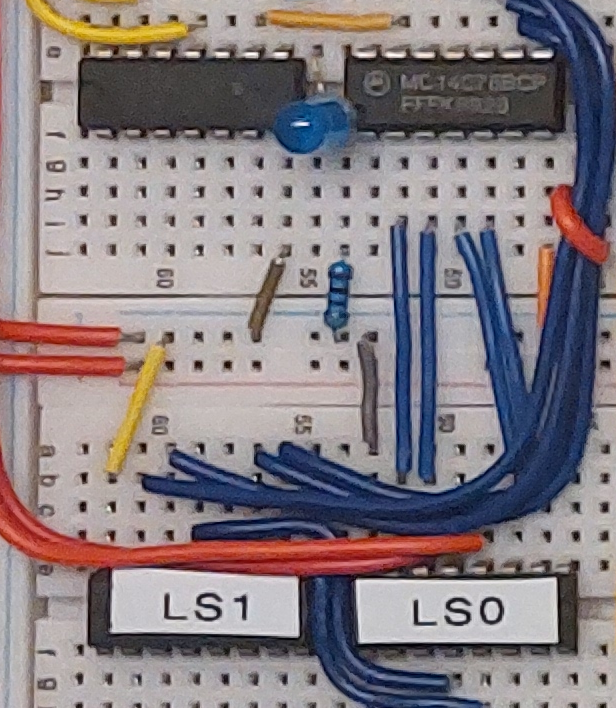
\includegraphics[width=0.3\textwidth]{img/lsregistercloseup}
  \caption{Close up of the Loop Skip Register Module.}
  \label{fig:spregcloseup}
\end{figure}

\subsubsection{Overview}
The Loop Skip Register (LS) is used to produce the loop-skip-flag (S, see \ref{sec:architecture:ls}). It is implemented using two 74LS193 binary counters and is connected to register driver at address 5 (0b101). Like the Z-flag, the S-flag is produced by sending the outputs of the binary counters through an 8-input NOR-gate, the output of which is then inverted and connected to the FB flag-register. When any of these bits are high, the S flag will be raised, indicating that the computer is in the process of skipping the current loop.


\subsubsection{Schematic}
A full schematic is provided on the next page.
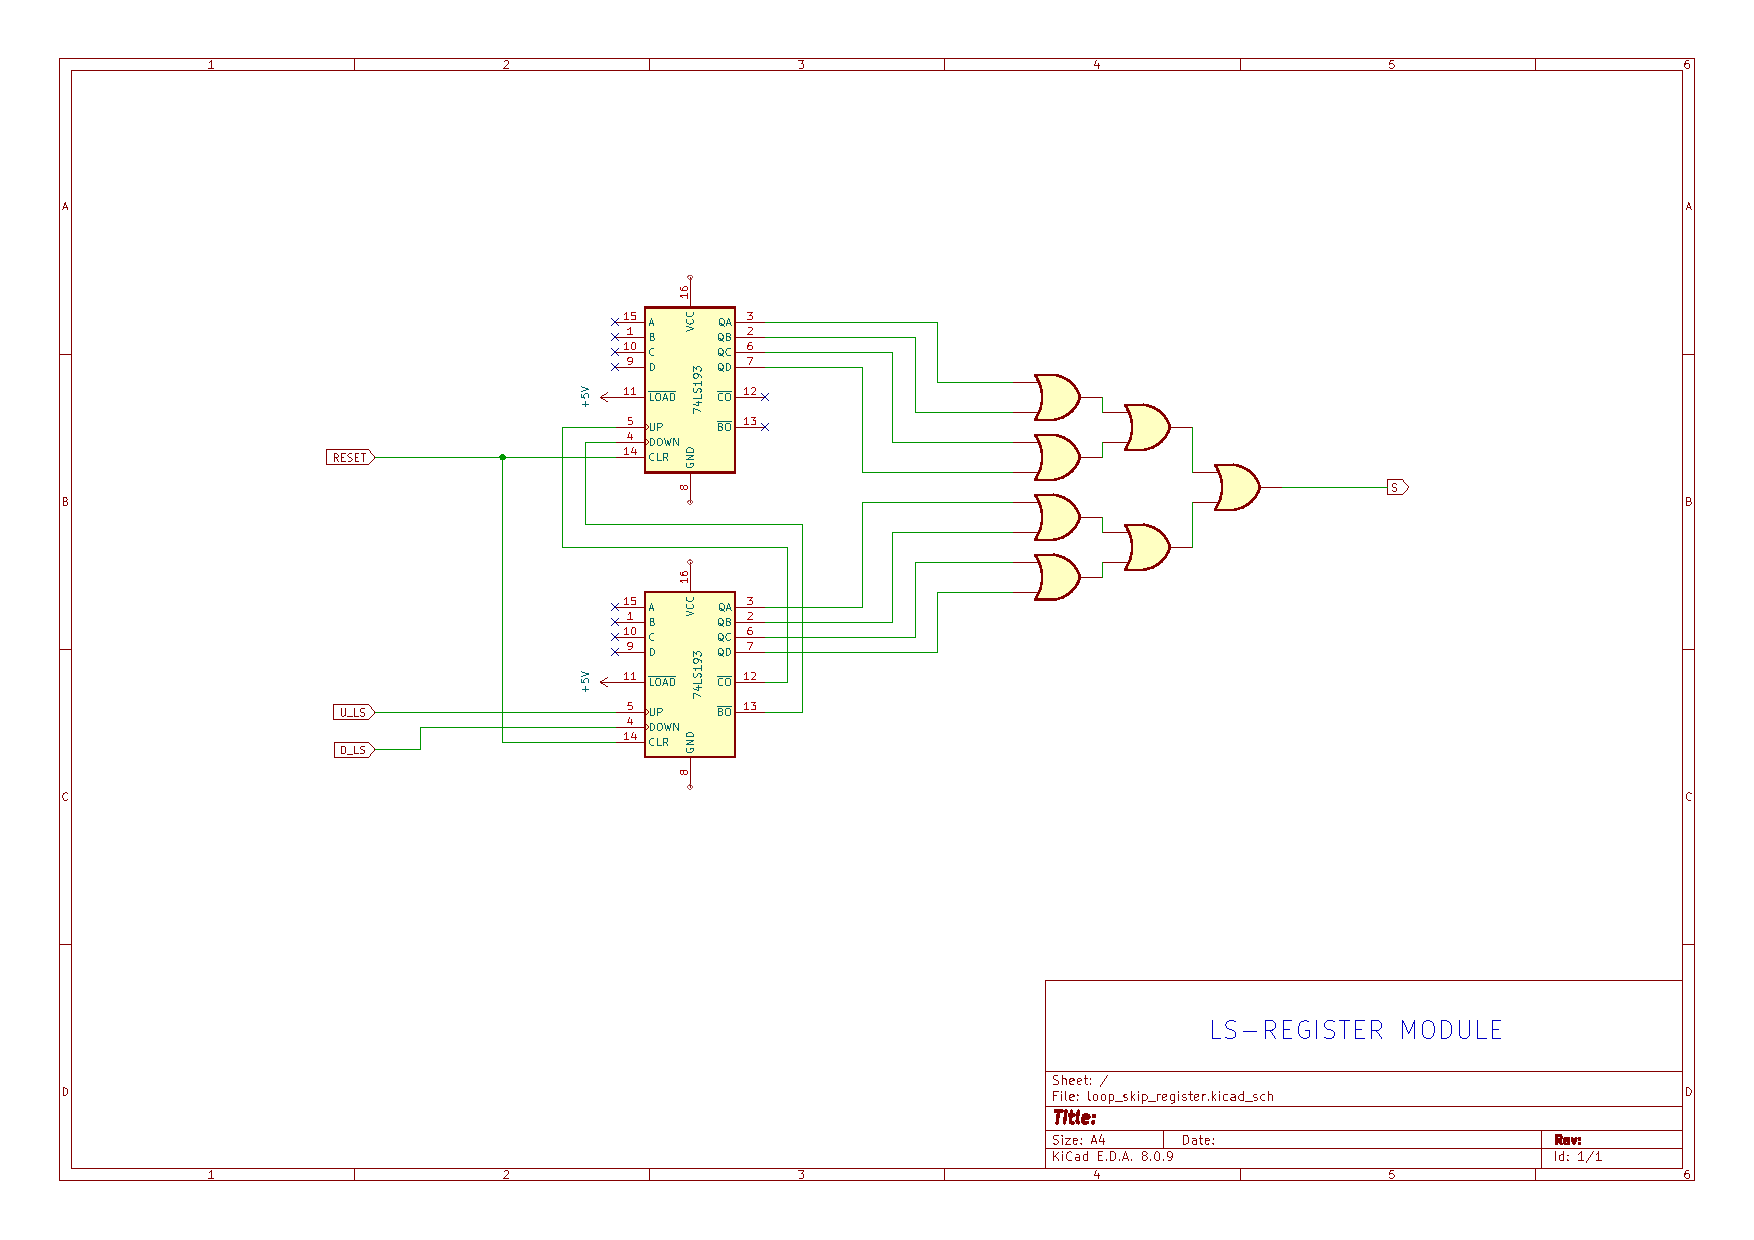
\includepdf[landscape=true]{schematics/loopskipregister.pdf}


%%%%%%%%%%% FA/FB

\subsection{Flag Registers}
\begin{figure}[H]
  \centering
  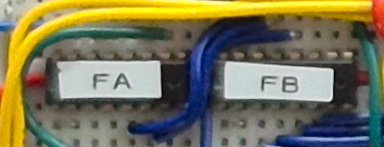
\includegraphics[width=0.6\textwidth]{img/flagregistercloseup}
  \caption{Close up of the flag registers FA and FB.}
  \label{fig:ramcloseup}
\end{figure}

\subsubsection{Overview}
There are two stages of flag-buffering; the first stage is the FA register (in which the A and V flags are stored) and the second the FB register (in which all flags except K are latched when the instruction is loaded). Both of these registers have been implemented using a 74LS173 4-bit register. The A and V flag are stored in FA by the CU whenever the value in D is changed (V) or whenever the pointer is changing its position (A). This can happen mid-instruction without changing the address on the microcode EEPROMs because the flag lines leading into those come from the FB register. At each cycle 0, the buffered A and V flags are loaded into FB, together with S and Z coming from the LS and D registers respectively. Since this always happens in conjunction with loading the instruction from program ROM into the instruction register (see \ref{sec:implementation:cu}), the control signal has been named LD\_FBI. The flags in the FB register will (mostly) remain constant during the execution of an opcode.

\subsubsection{Schematic}
A full schematic is provided on the next page.
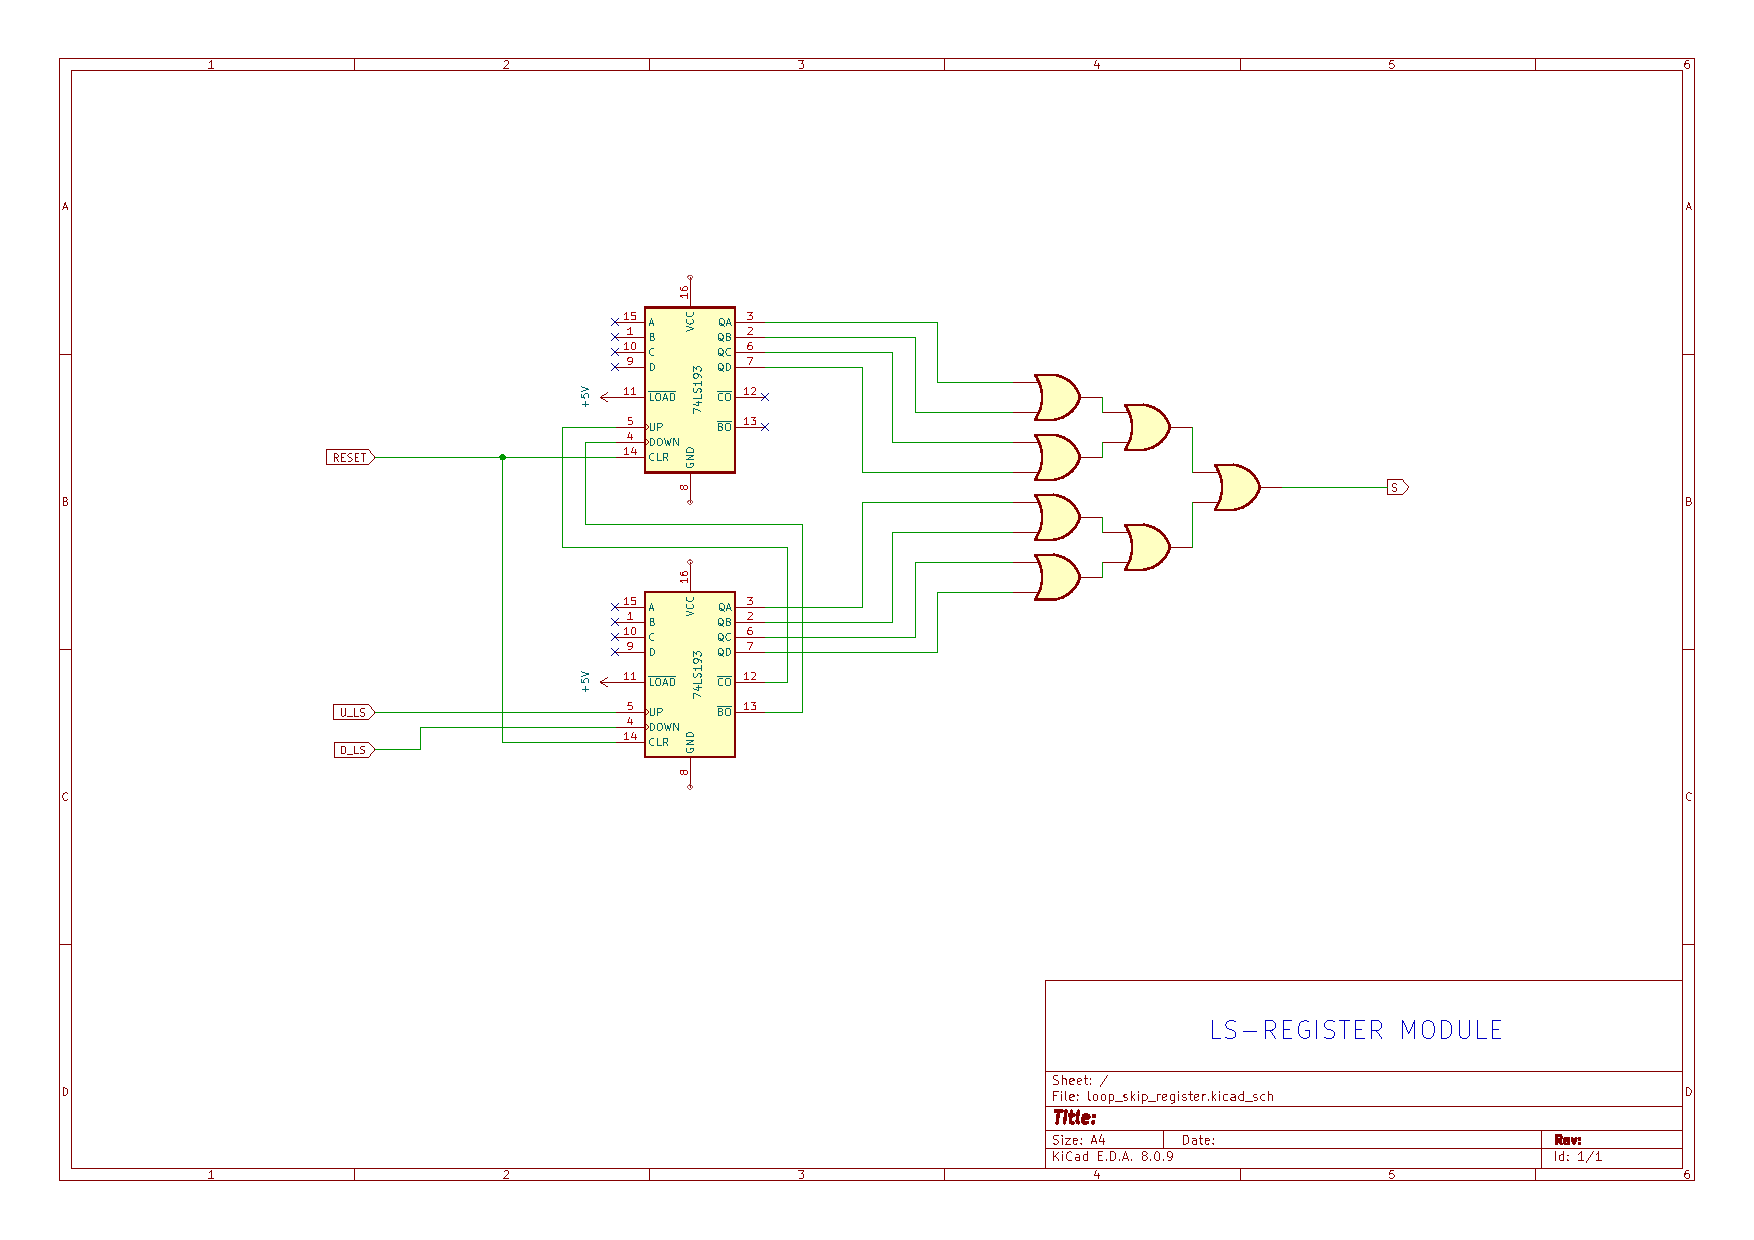
\includepdf[landscape=true]{schematics/loopskipregister.pdf}


%%%%%%% RAM Module

\subsection{RAM}
\begin{figure}[H]
  \centering
  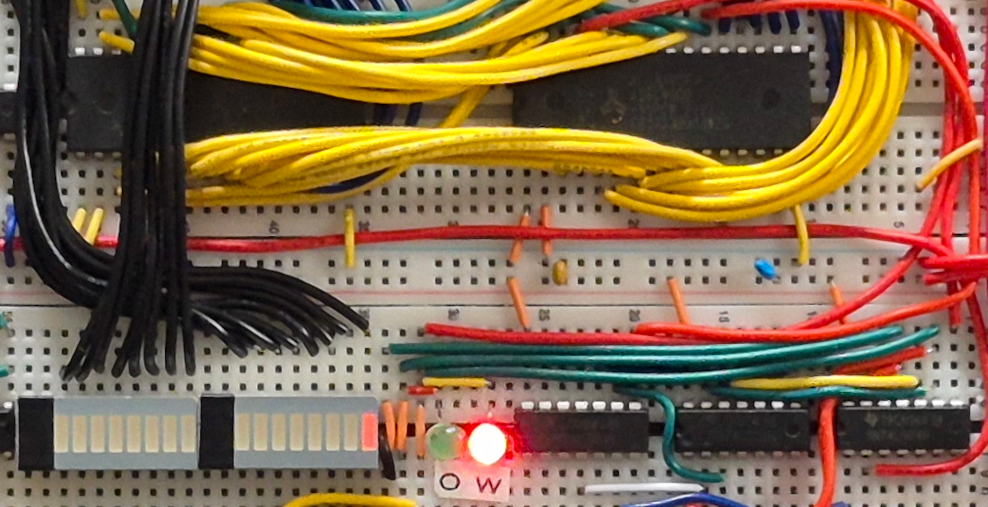
\includegraphics[width=0.6\textwidth]{img/ramcloseup}
  \caption{Close up of the RAM Module.}
  \label{fig:ramcloseup}
\end{figure}

\paragraph{Capacity} The RAM module is mainly used to store the 8-bit data of the BF memory-tape. However its secondary purpose is to also store the instruction-pointer values when loops are handled, which are 16-bit in size. Therefore the RAM module contains two 512K x 8-bit SRAM chips (AS6C4008) for a total of 512K 16-bit memory-cells. The second chip is therefor only used to store the high-byte of the IP's stored on the stack (at most 256 values). The remainder of the capacity of this chip is not used at all, since the datavalues are only 8 bits in size.

\paragraph{Buffering} The AS6C4008 already provides a Chip Enable input which is supposed to be used when the data is connected to a databus. When this input is inactive, its outputs are in a high impedance state to avoid bus contention with other devices. However, in this project we need the data currently pointed to to be visible on an array of LED's, which means that the chip should be enabled basically at all times (except when writing to it). Additional logic is used in conjunction with a pair of 74LS245 tristate buffers to intercept the outputs before making them available on the bus through the buffers. The truthtable for this logic is incorporated in the schematics below. The LED's are not shown in the schematic, but can be connected directly to the datalines of the RAM in this configuration. 

\subsubsection{Schematic}
A full schematic is provided on the next page.
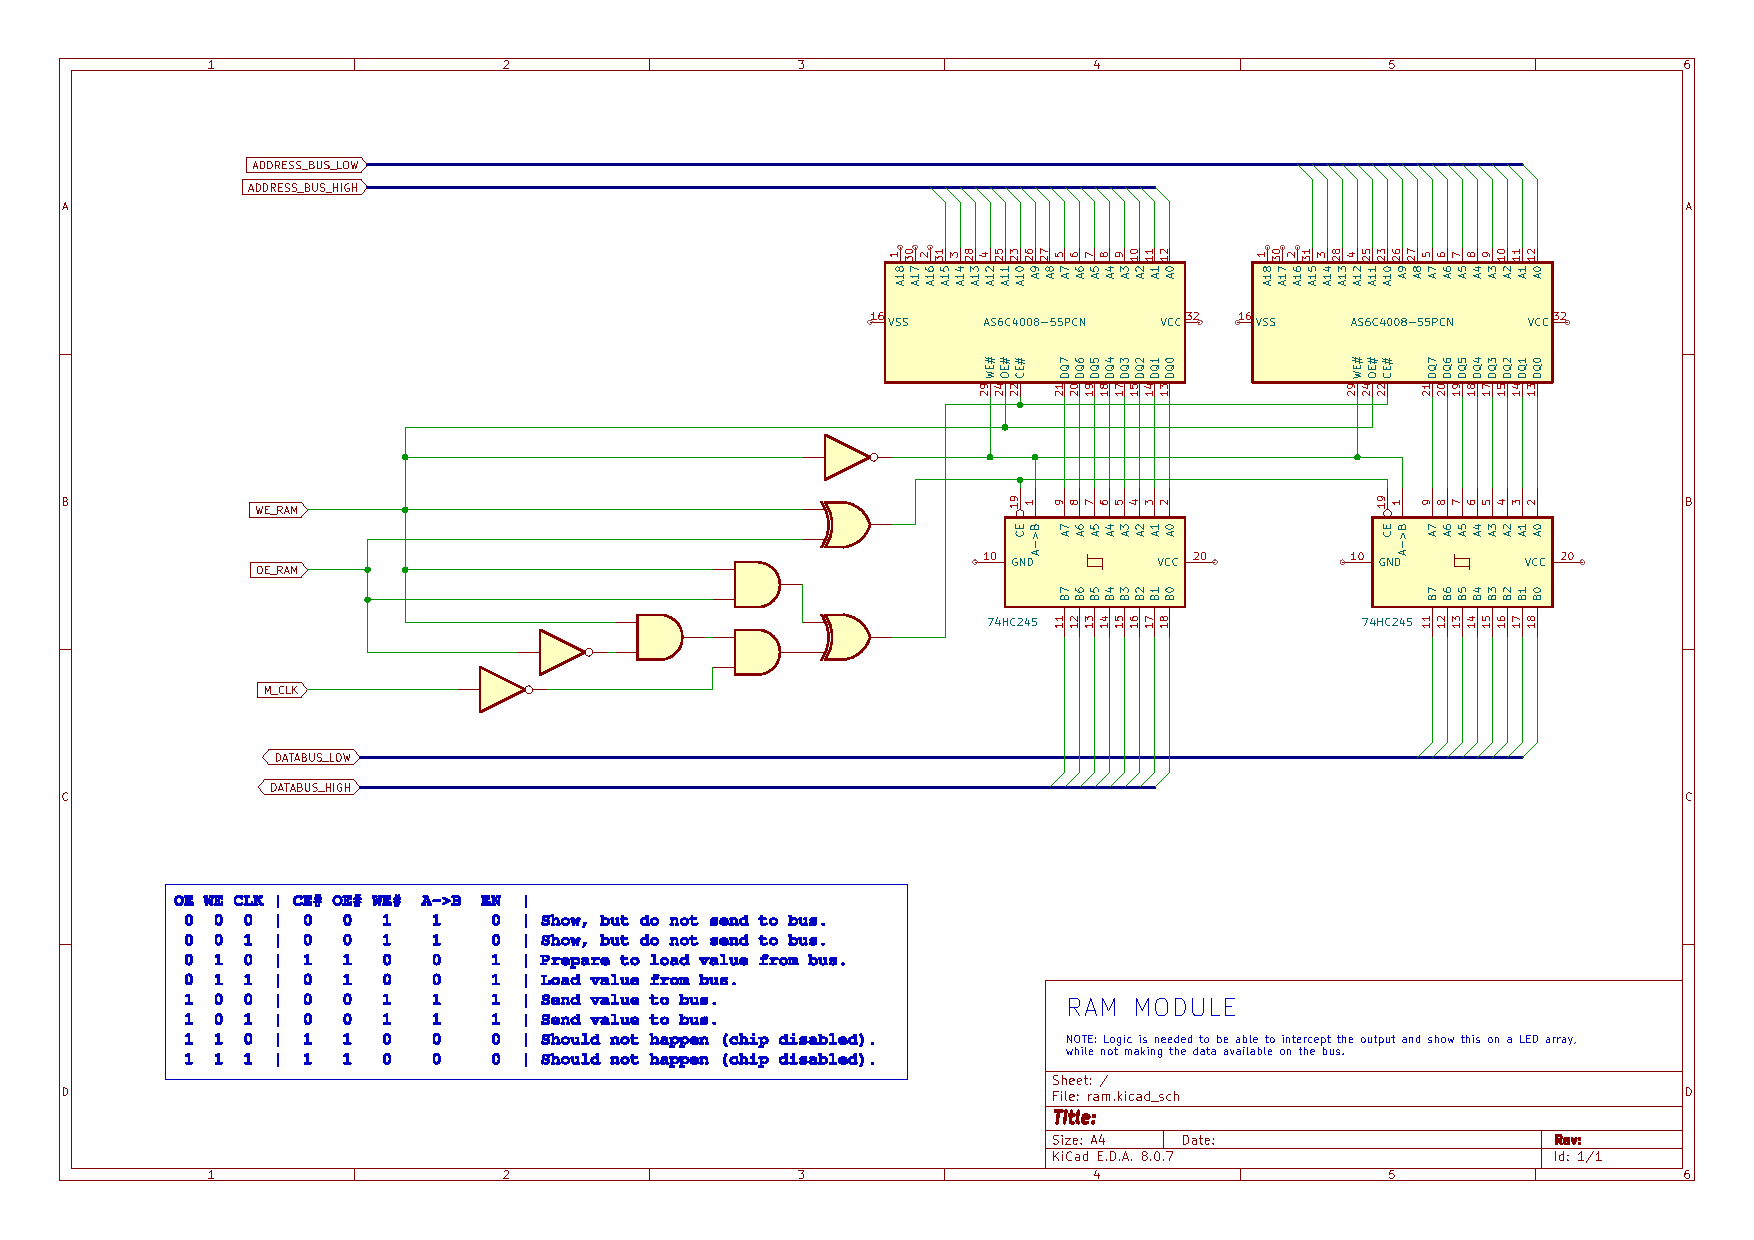
\includepdf[landscape=true]{schematics/rammodule.pdf}


%%%%%%% CONTROL UNIT

\subsection{Control Unit}\label{sec:implementation:cu}
\begin{figure}[H]
  \centering
  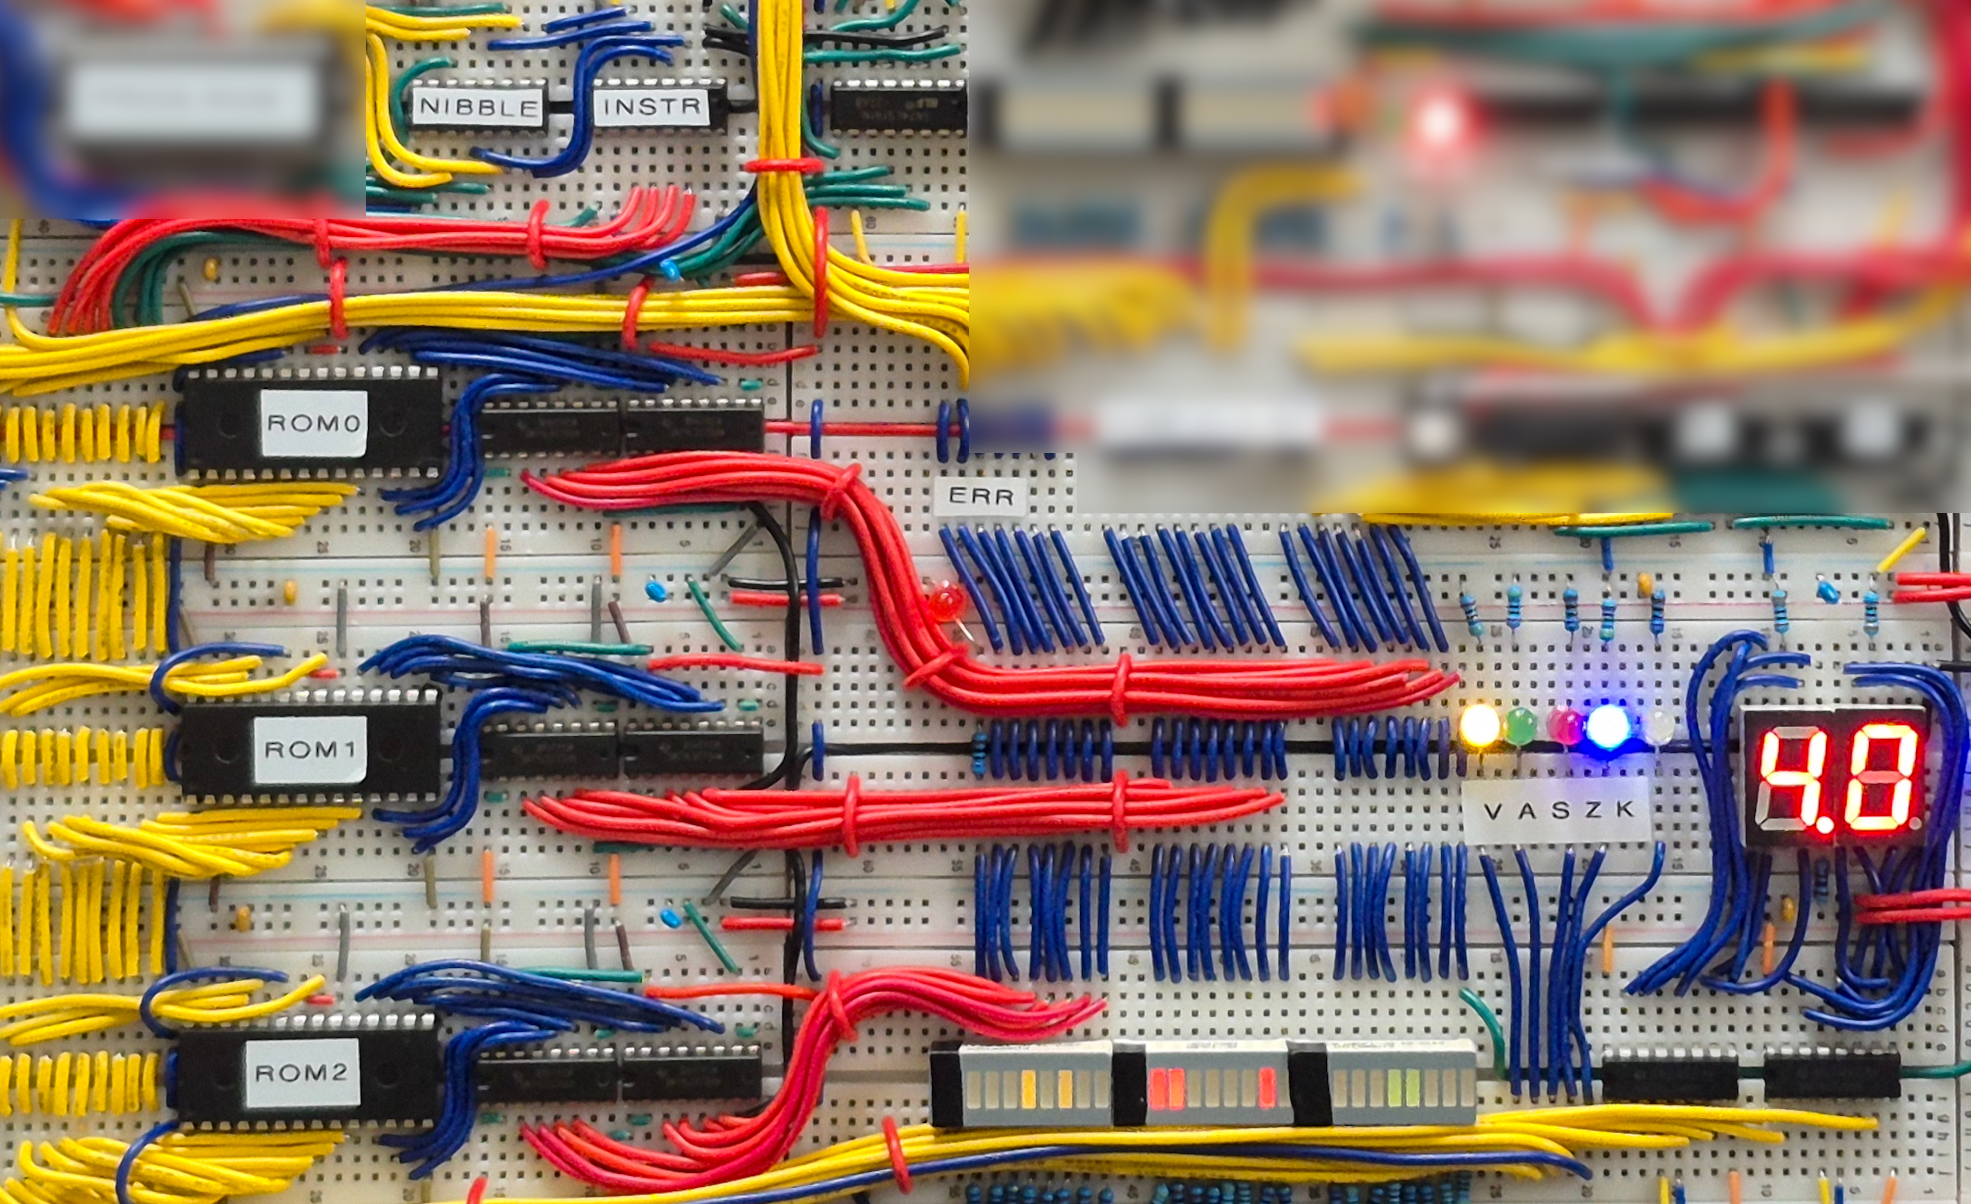
\includegraphics[width=0.6\textwidth]{img/controlunitcloseup}
  \caption{Close up of the Control Unit.}
  \label{fig:controlunitcloseup}
\end{figure}

\subsubsection{Overview}
The control unit is responsible for sending the appropriate control-signals to each of the modules. The general idea is that the current instruction pointed to by the IP (4 bits) together with the state flags (another 5 bits: K, A, V, S and Z) and the cycle count (3 bits) combine together to form a 12-bit address into a set of three EEPROM chips (AT28C64B), each of which contains part the signal configuration corresponding to the current state of the system. When clocked by the decoder-clock (D\_CLK), the values currently at this address are loaded into six 74LS173 registers (two per EEPROM) and asserted onto their respective modules, which will act upon them on the next pulse of the M\_CLK signal.

\paragraph{Address Layout.} Based on the physical layout of the board, the following configuration was used to construct an address into the EEPROMs.
\\
\begin{center}
\begin{tabular}{r|ll} 
  Address Bits & \\ \hline
  0-2  & Cycle count & ($000_2$ - $111_2$) \\
  3-7  & Instruction & ($0000_2$ - $1111_2$) \\
  8-12 & Flags  & ($00000_2$ - $11111_2$) \\
  13   & Unused & 
\end{tabular}
\end{center}


\paragraph{Generating and Programming Microcode.} The three EEPROM's have been programmed using a custom built EEPROM programmer based around an Arduino Nano, combined with a python script (\texttt{bflash.py}) that is able to send a binary image to the Nano over a serial connection. The images that store the microcode tables have been generated by Mugen (see \ref{sec:utilities:mugen}), a utility developed to make the microcode programming more maintainable. Mugen generates the images from a specification file. The relevant part of the specification for the Synapse-191 is shown in the listing below and is a direct representation of the microcode shown in Table \ref{tab:microcode}.

\newpage
\lstinputlisting[style=MugenStyle, firstline=58, firstnumber=1]{../src/microcode/bfcpu.mu}


\paragraph{Instruction Nibbles.} The actual BF program is stored in another 8K EEPROM chip (AT28C64) and is addressed by the instruction pointer as mentioned before. Since each BF instruction only needs 4 bits to be encoded (there are less than 16 different opcodes), we can store up to 16K instruction in the chip by packing 2 consecutive instructions together in a single byte (handled by the assembler, \texttt{bfasm}). Rather than using bit 0 from the IP directly as address bit 0 on the EEPROM, it is used as the data-select signal to a 74LS157 multiplexer. This multiplexer takes 1 select-bit and two sets of 4 databits. Depending on the value of the select-bit, one of the sets of 4-bit data is sent to its outputs. This allows us to select either the low or high nibble of the data in the EEPROM, effectively doubling the amount of instructions that can be stored and retrieved.

\paragraph{Instruction Register.} The seleted nibble is loaded into the instruction register (I) at the same time as the V, A, S and Z flags are loaded into the FB register. For this reason both the FB and I registers can operate on the same control-signal: LD\_FBI. The I register is implemented using the 74LS161, which is actually a counting register, because at the time there was no '173 available anymore and these chips are functionally almost identical when counting is disabled on the '161. Initially, the outputs of the multiplexer ('157) were directly connected to the address lines of the microcode EEPROMs but when it turned out that this could cause instabilities in some rare occasions, the I register was added to buffer the instruction for the entire duration of the opcode execution.
 
\paragraph{Cycle Counter.} The cycle counter is implemented by a 74LS161 binary counter that simply increments on every M\_CLK signal up and sends its outputs (bits 0-2) to address lines 0-2 of the microcode EEPROM chips. It is reset when it receives the CR signal (which becomes active when after an instruction has completed).


\subsubsection{Schematic}
A full schematic is provided on the next page.
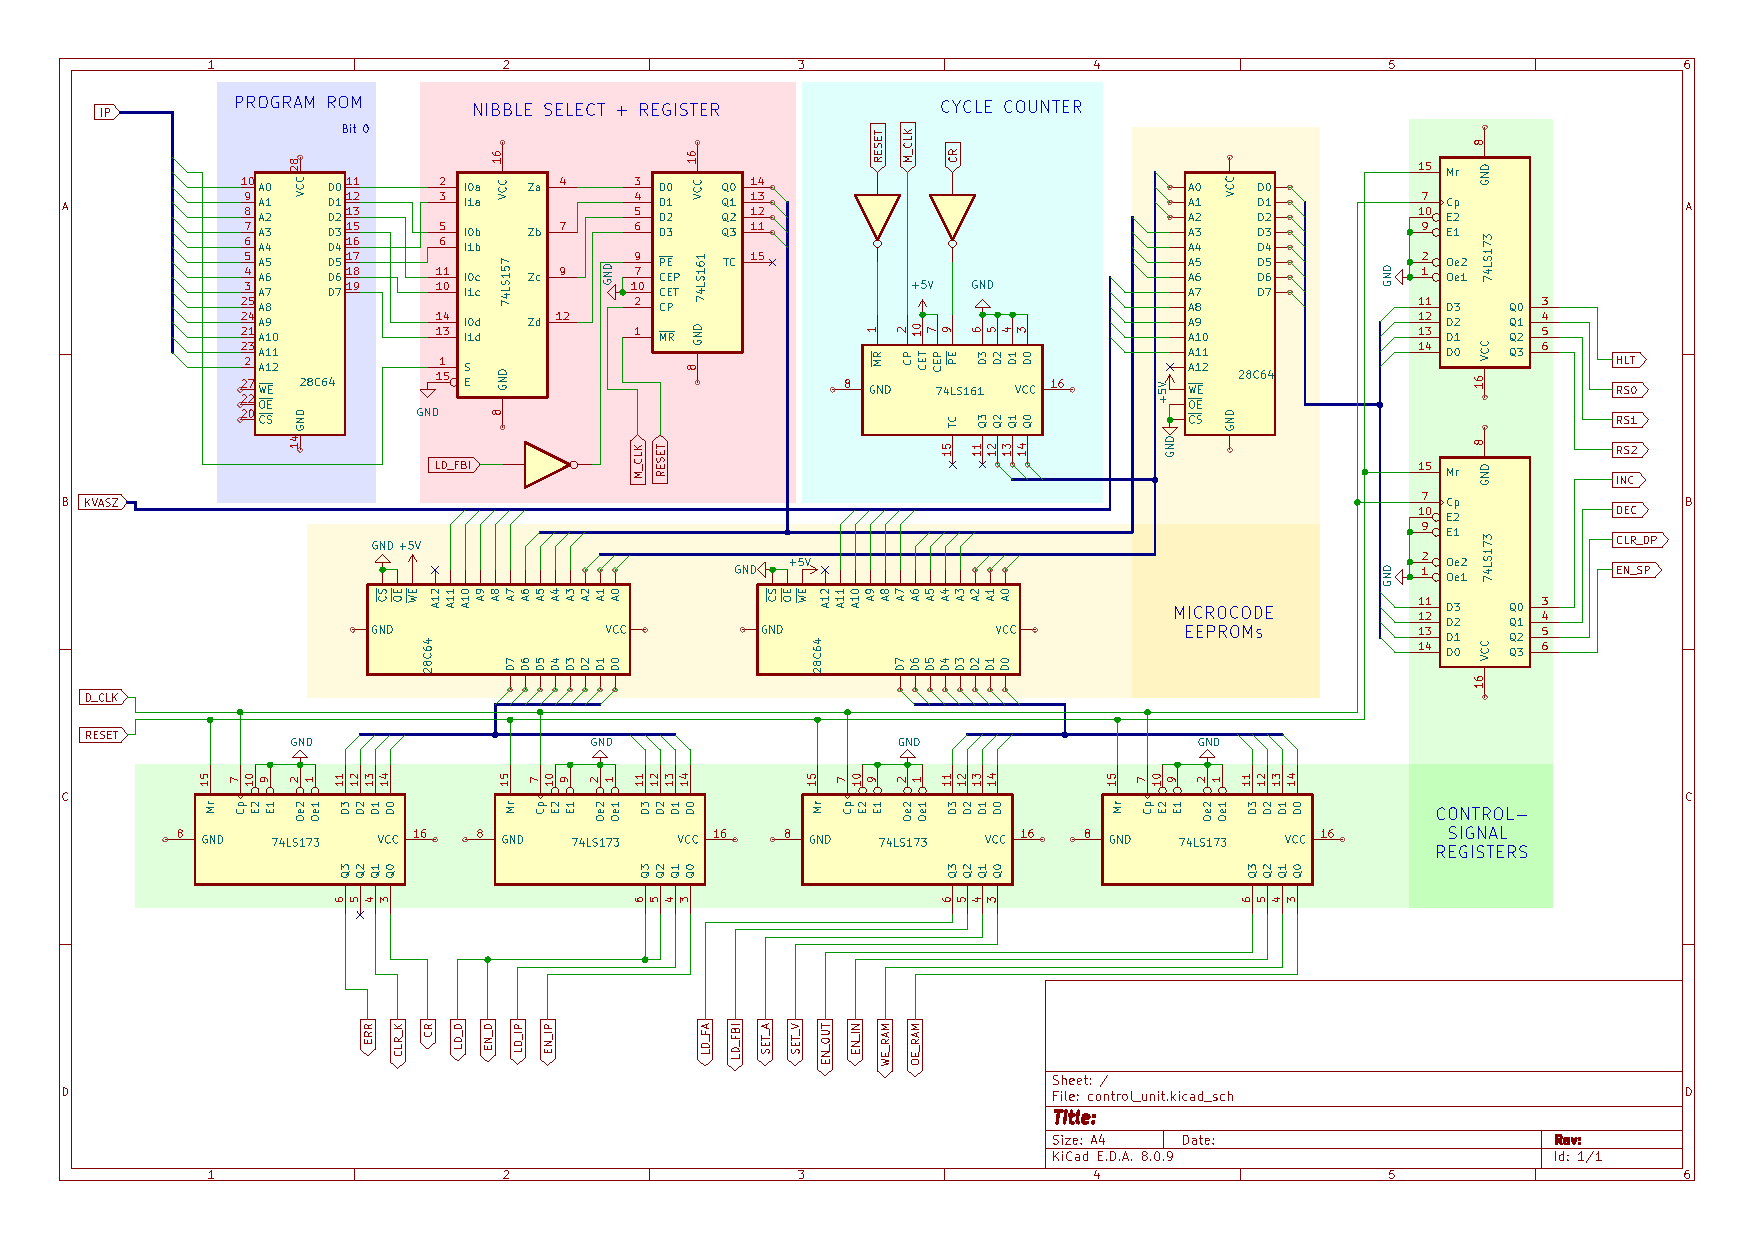
\includepdf[landscape=true]{schematics/controlunit.pdf}

%%%%%%% IO Module
\subsection{IO Module} \label{sec:implementation:io}
\begin{figure}[H]
  \centering
  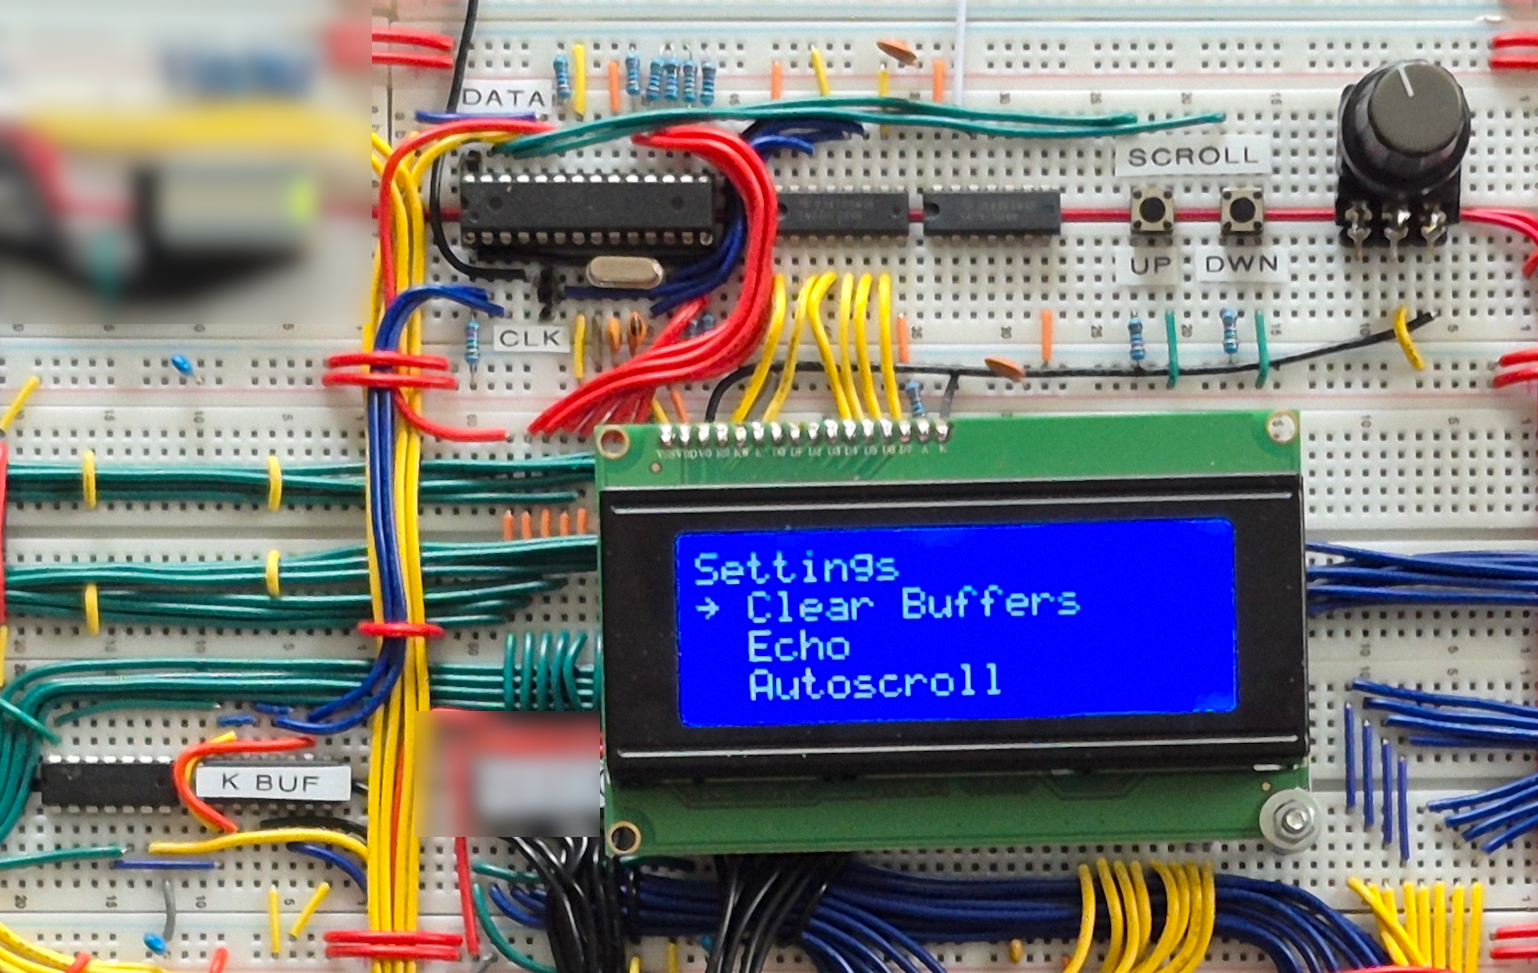
\includegraphics[width=0.6\textwidth]{img/iomodulecloseup}
  \caption{Close up of the IO Module.}
  \label{fig:iomodulecloseup}
\end{figure}

\subsubsection{Overview}
The IO system is handled by an ATMEGA328P microprocessor, commonly found in the Arduino Uno. It has four main functions:
\begin{enumerate}
\item Drive the screen and display contents from the bus when instructed to by the \texttt{EN\_OUT} signal.
\item Handle keyboard input and provide input data to the bus when instructed to by the \texttt{EN\_IN} signal.
\item Provide a random number to the bus when both signals are supplied (implementing the \emph{Random Brainf*ck Extension}).
\item Supply a menu system to alter its settings using two buttons.
\end{enumerate}

\paragraph{Buttons and Menu} Two buttons are provided to interact with this system. They are mainly used to scroll the screen but can also be used to access and navigate a menu (Figure \ref{fig:menuscreen}). This menu let's the user do the following:
\begin{enumerate}
\item Clear the screen and keyboard buffer.
\item Change the display-mode. By default, incoming data is interpreted as ASCII characters. When it should be displayed as raw numerical values (either in base 10 or 16), this option can be selected from the menu. When in either of these numerical modes, a delimiter character can be selected to separate bytes visually.
\item Set autoscrolling on/off. By default the screen will scroll its contents when they overflow to always keep the most recent data in view. When new data is displayed, the screen is always scrolled to display this data. Setting autoscroll to `off' will disable these features.
\item Echo on/off. When running an interactive program that requires keyboard input, the user probably wants to see what is being typed. This is the default behavior (echo on). If for some reason the keypresses should not be displayed, this option can be disabled.
\item Set the input-mode. By default, the IO module will wait for the input-buffer to contain a value before putting anything on the bus and notifying the CU throught the K-flag (buffered input-mode). However, an alternative mode (immediate) can be selected, in which case the IO module will put a zero on the bus when the buffer is empty and set the K-flag regardless. This can be helpful if programs require real-time inputs (e.g. for simple games).
\item Set the RNG seed. For programs that use the Random Number Generator as an input device, the seed can be set through this option. Since the same seed will produce the same sequence of numbers, this option can be used to control the randomness of the application. A `true' random seed can normally be emulated by seeding the generator with the reading of a floating analog input for example, but sadly no free analog inputs were left available on the MCU.
\item Reset to default settings. Whenever settings have been changed, the new settings will be saved to the persistent EEPROM memory of the MCU and loaded back on startup to make the settings persist when the MCU is powered down. This option allows you to revert all changes and load the default settings back in.
\end{enumerate}

\begin{figure}[h]
  \centering
  \includegraphics[width=0.5\textwidth]{img/menuscreen}
  \caption{Part of the menu that is accessible by pressing both scroll-buttons simultaneously.}
  \label{fig:menuscreen}
\end{figure}


\subsubsection{Handshake Protocol}
\paragraph{Output} The \texttt{M\_CLK} signal is connected to an interrupt pin of the MCU. On every interrupt triggered by the clock, when the system is in its IDLE state, it will check the EN\_IN and EN\_OUT lines to determine if it should initiate a read or write sequence to the databus. When EN\_OUT is found to be high, it will copy the byte currently present on the bus into its screen-buffer, set the K flag and change its state to WAIT\_SYS. On every subsequent clock pulse, while in the WAIT\_SYS state, it will check if the K flag has been reset by the control unit. If so, the handshake has been completed and the module returns to its IDLE state (see Figure \ref{fig:isrflow}).

\paragraph{Input} If the EN\_IN signal is found to be asserted, the system has two possible courses of action, depending on the input-mode currently set by the user (through the on-screen settings menu). In (the default) buffered mode, the system will change its state to WAIT\_KB and wait for a byte to become available in the keyboard-buffer. As soon as it does, it will provide this value onto the bus and notify the CU by setting the K flag. It then moves into the WAIT\_SYS state to await confirmation by the CU (which in turn resets the K flag). In immediate mode, all zeros will be written to the bus and the K flag is set immediately even when the keyboard-buffer is still empty. If, in addition to EN\_IN, EN\_OUT is asserted as well, a random byte is put onto the bus (see Figure \ref{fig:isrflow}).

\begin{figure}[H]
  \centering
  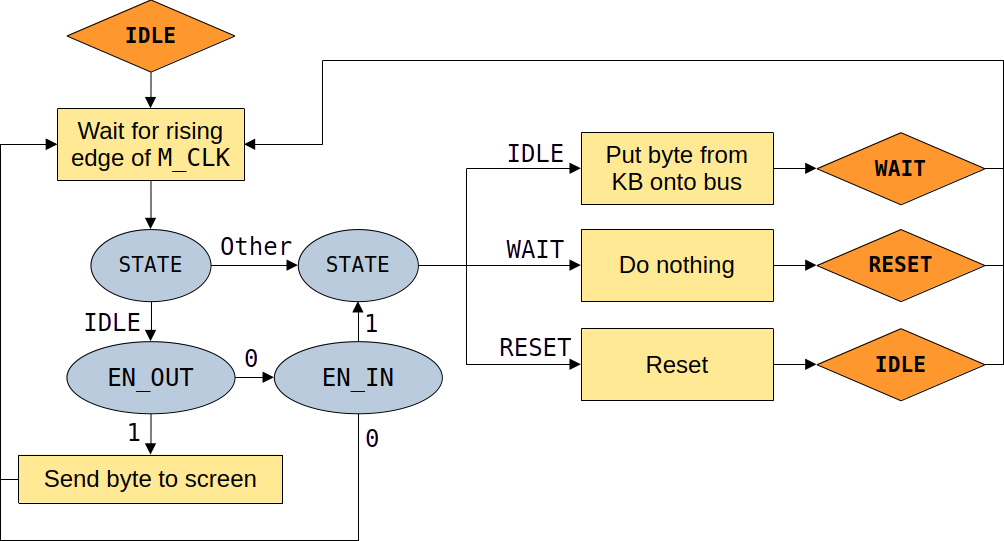
\includegraphics[width=\textwidth]{img/isrflow}
  \caption{Control flow inside the ISR running on the microcontroller.}
  \label{fig:isrflow}
\end{figure}

\subsubsection{Shift Register}
A shift register (74HC595) had to be used to decrease the number of pins on the Atmega328p necessary to drive the LCD screen. Not a single IO pin has not been used, so the shift register proved invaluable for this application.

\subsubsection{LCD Screen}
The software was written in such a way that most common LCD character screens (compatible with Hitachi the HD44780 driver) will be handled appropriately. Both a 16x2 and 20x4 have successfully been installed in the computer. A modified version of the \texttt{LiquidCrystal\_74HC595} library was used to implement the LCD driver.

\subsubsection{Keyboard}
The IO module can only handle input from PS/2 compatible keyboards. A modified version of the \texttt{PS2Keyboard} library was used to implement the keyboard driver.


\subsubsection{Schematic}
A full schematic is provided on the next page.
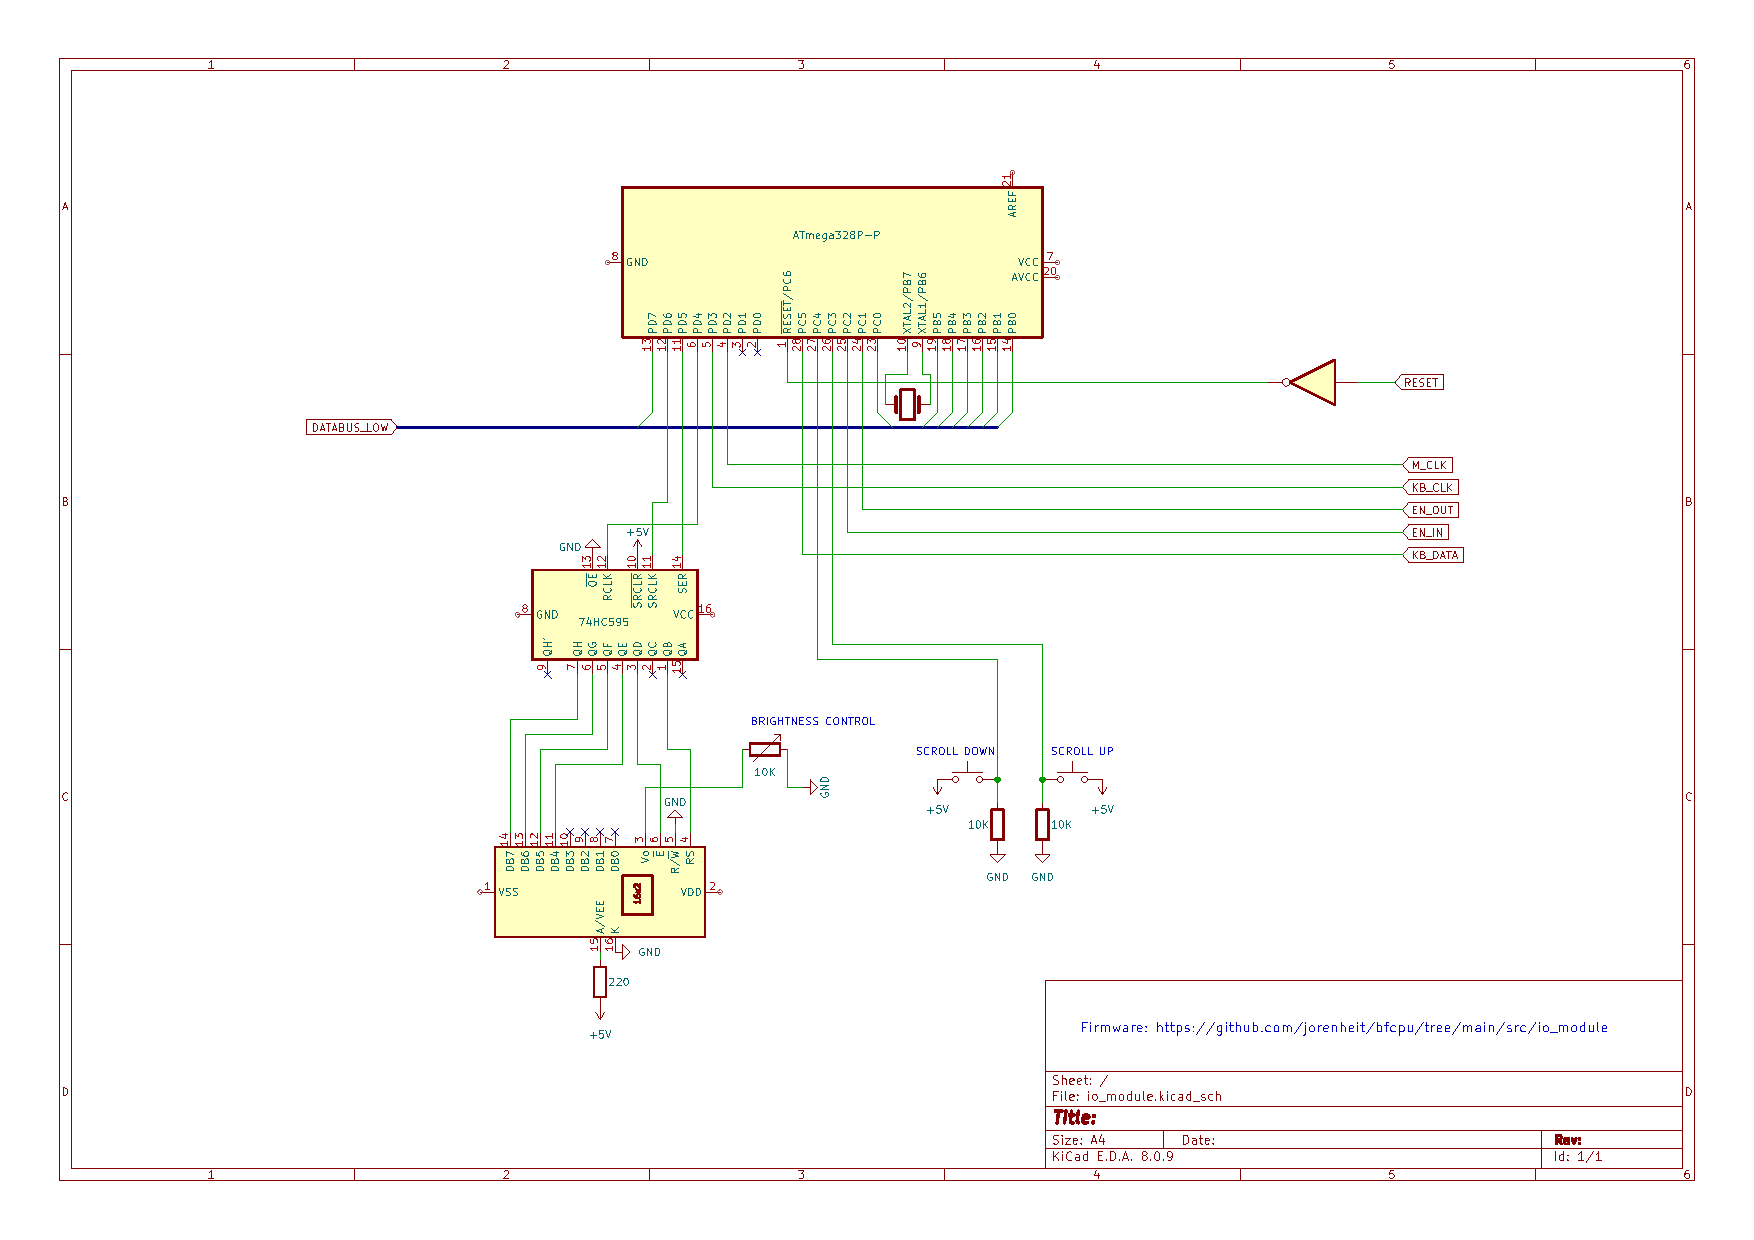
\includepdf[landscape=true]{schematics/iomodule.pdf}


\subsection{IO Module Firmware}
To ensure minimal latency and efficient CPU--peripheral communication, several low-level optimizations were applied to both the interrupt routine and the main execution loop of the module's firmware. 

\subsubsection{Ring Buffers}
\paragraph{Overview} The IO module employs a set of custom ring buffers that provide high-speed, non-blocking data transfer between the asynchronous microcontroller firmware and the synchronous TTL-based CPU. The ring buffer (or circular buffer) is a fixed-size, first-in-first-out (FIFO) data structure that uses two indices, commonly called the \texttt{head} and \texttt{tail}. The \texttt{head} marks the position where the next incoming element will be written, while the \texttt{tail} indicates the position of the next element to be read. When either index reaches the end of the buffer, it wraps around to the beginning, forming a logical ring in memory. This structure eliminates the need for memory allocation or data shifting, providing constant-time access for both enqueue and dequeue operations. See Figure \ref{fig:ringbuffer}.

\begin{figure}[H]
  \centering
  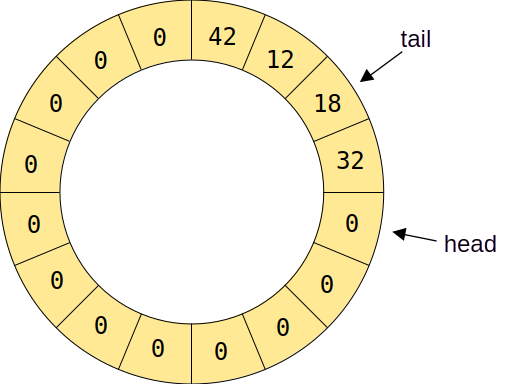
\includegraphics[width=0.3\textwidth]{img/ringbuffer}
  \caption{In this ring buffer, the value 18 (pointed to by \texttt{tail}) will be returned on the next query. Data entering the ringbuffer will be stored at the cell pointed to by \texttt{head}. The value 42 is the first value to be overwritten when the \texttt{head} pointer wraps around to the top of the buffer.}
  \label{fig:ringbuffer}
\end{figure}


In the Synapse-191 I/O module, one ring buffer is dedicated to temporaroly storing incoming data (bytes coming from the CPU that need to be written to the LCD screen), the screen-buffer, and another is used for outgoing data (keyboard input that needs to be put on the data bus), the keyboard-buffer. The main loop periodically flushes the screen-buffer to the display and refills the keyboard-buffer with new data when it arrives. Meanwhile, the interrupt service routine (ISR) accesses these buffers asynchronously to satisfy CPU read and write requests. Since all the heavy lifting (interpreting incoming data, managing the LCD screen, decoding keyboard scan-codes) is done in the main-loop, the ISR is kept very compact.

\paragraph{Optimizations} The ring buffer is implemented as a templated C++ class, parameterized by buffer size and value type. Several compile-time and runtime techniques were employed to maximize performance and memory efficiency. A combination of compile-time specialization and minimal arithmetic overhead allows the ring buffers to perform deterministic, low-overhead enqueue and dequeue operations, which is essential for keeping up with the `high' frequency external system clock of the Synapse-191 CPU.

\begin{itemize}
\item \textbf{Index Type Specialization:} The index-type (datatype used to store the \texttt{head} and \texttt{tail} indices, is selected automatically at compile time using template metaprogramming. For small buffers, 8-bit indices are used instead of 16- or 32-bit counters, reducing instruction count, register usage and thus ensuring the fastest possible integer operations on out 8-bit MCU.
\item \textbf{Integer Wrapping Optimization:} For buffers that are exactly as big as the maximum number representable by some type, that type is used to index the buffers as per the logic above. For example, a 256 byte buffer can be indexed fully using an 8-bit type like \texttt{unsigned char}. A value of 255 represented by this type will automatically wrap around when incremented, rendering any additional modular arithmetic to wrap around to the start of the buffer unnecessary.
\item \textbf{Power-of-Two Optimization:} When the buffer size does not match the condition above, but \emph{is} a power of two, the modulo operation used for index wrapping is replaced with a simple bitwise \texttt{AND} operation: \texttt{i -> (i + 1) \& (N - 1)}. This reduces the naive modulo operation from multiple CPU cycles to a single instruction.
\end{itemize}

\paragraph{Volatile Access and Memory Barriers} The \texttt{head}, \texttt{tail}, and data array are declared \texttt{volatile} to prevent compiler reordering and ensure consistency between the ISR and the main loop. Additionally, an inline assembly memory barrier guarantees that writes to the buffer are completed before the corresponding index is updated, avoiding race conditions.

\subsubsection{Direct Port Access} The ISR itself is further optimized using \emph{direct port manipulation}. Instead of relying on Arduino’s \texttt{digitalRead()}, \texttt{digitalWrite()} and \texttt{pinMode()} functions, which incur significant overhead, the firmware performs raw register accesses (\texttt{PORTX} for writing \texttt{PINX} for reading and \texttt{DDRX} for setting their modes) through custom inline functions. This facilitates faster control over timing-sensitive pins.

\subsubsection{Compile-time Menu Structure} Finally, the on-screen configuration interface uses a statically defined menu tree that is fully constructed at compile time using template metaprogramming techniques. This eliminates dynamic memory allocation and object initialization overhead during runtime, minimizing both execution latency and memory footprint. Together, these optimizations produce a maintainable, fast, and memory-efficient IO subsystem capable of operating reliably at high clock speeds of the CPU core.
\vfill
\lstinputlisting[language=c++,firstline=65,lastline=99,firstnumber=1]{../src/io\_module/lcdmenu.h}
